\section{Blinks} \label{chap:blinks}

\subsection{From blackboard framed links to blinks}
\label{sec:BFL2Blinks}

In Section \ref{sec:bfl} we saw that a blackboard framed link or BFL
is a link diagram that induces a space. We now describe a procedure
to build a new object from a blackboard framed link.

\begin{figure}[htp]
   \begin{center}
      \leavevmode
      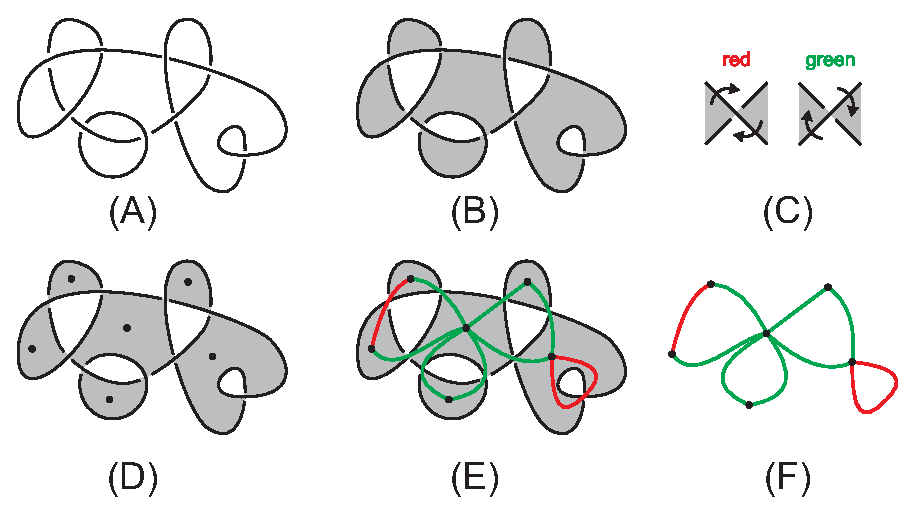
\includegraphics[width=12.5cm]{A.figs/bfl2blink.eps}\\
   \end{center}
   \vspace{-0.7cm}
  \caption{Procedure \textsc{BFL2Blink}}
  \label{fig:BFL2Blink}
\end{figure}

Follow the steps described in this paragraph on the example of
Figure~{\ref{fig:BFL2Blink}}. Start with a BFL
(Figure~{\ref{fig:BFL2Blink}A}). We say that two faces on a BFL are
{\it adjacent} if they share a curve (not just a point) that
separates them. The faces of a BFL can be colored black or white
such that no two adjacent faces have the same color. To do this
first define all faces as {\it unassigned}: no color. Then assign
white to the external face of the BFL. Then repeat this: assign
white a face that is adjacent to a black face or assign black a face
that is adjacent to a white face, until all faces are assigned white
or black. This procedure always leads to a unique coloring.
Figure~{\ref{fig:BFL2Blink}B} shows the resulting color assignment
of the BFL of Figure~{\ref{fig:BFL2Blink}A} with the black faces
painted in gray and white faces painted white. The next step is to
classify each crossing of the BFL as {\it red} or {\it green}
(Figure~{\ref{fig:BFL2Blink}C}). A crossing is {\it red} if the
overcrossing line, on the clockwise direction, separates a black
face from a white face. A crossing is {\it green} if the
overcrossing line, on the clockwise direction, separates a white
face from a black face. Now choose one interior point on each black
face as shown in Figure~{\ref{fig:BFL2Blink}D}. For each crossing
$c$, let $A$ and $B$ be the chosen interior points of the two black
faces involved in $c$. Draw a simple curve from $A$ to $B$ such
that: (1) it passes through the crossing point of $c$; (2) all of its
points are black region points or the crossing point of $c$; (3) its
points that are not end-points do not intersect any other crossing
curve. Note that $A$ and $B$ can be the same point. In this case the
curve is a {\it loop}. Figure~{\ref{fig:BFL2Blink}E} shows the
result after drawing all such curves. Figure~{\ref{fig:BFL2Blink}F}
shows the new object after erasing the underlying BFL that guided
its construction. This resulting object is named a {\it blink} and
its general definition is a plane graph with each edge colored either red
or green. Note that a blink may have loops and multiple edges. Each
chosen point on each black face is called a {\it blink vertex} and
each simple curve is called a {\it blink edge}. The {\it size of a blink}
is its number of edges. The blink on Figure~{\ref{fig:BFL2Blink}F}
has size equal to 9.

We name the procedure described in last paragraph as
\textsc{BFL2Blink}. It is always possible to apply it in backwards
and obtain a blackboard framed link from a blink. So the
\textsc{BFL2Blink} when applied in backwards becomes the
\textsc{Blink2BFL} procedure. A blink and a BFL related by the
\textsc{BFL2Blink} or the \textsc{Blink2BFL} are said to be {\it
associated}. So the BFL on Figure~{\ref{fig:BFL2Blink}A} and the
blink on Figure~{\ref{fig:BFL2Blink}F} are associated.

\begin{figure}[htp]
   \begin{center}
      \leavevmode
      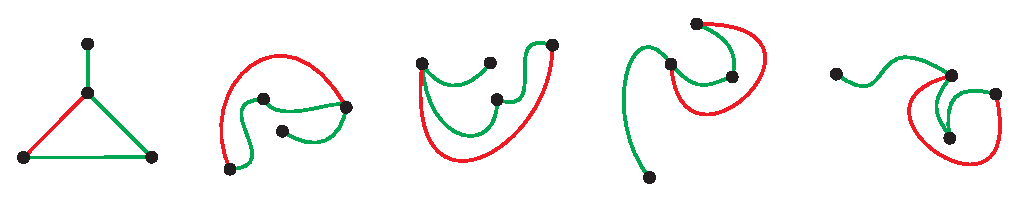
\includegraphics[width=9cm]{A.figs/blinksplaneisotopy.eps}
   \end{center}
   \vspace{-0.7cm}
   \caption{Blinks}
   \label{fig:BlinksPlaneIsotopy}
\end{figure}
In a strict sense, all blinks on Figure~\ref{fig:BlinksPlaneIsotopy}
are different. Their edges are different curves, so, as plane
graphs, they are different. But something connects all these blinks:
there exists a plane isotopy from any of these blinks to any other.
From now on, we say two {\it blinks are equal} if they are
``connected'' by a plane isotopy, otherwise they are {\it
different}. We use the same
convention with blackboard framed links: we say two {\it BFLs are
equal} if they are ``connected'' by a plane isotopy, otherwise they
are {\it different}.

We now claim that all associated BFLs of a class of equivalent
blinks (blinks connected by a plane isotopy) are also connected by
a plane isotopy and vice-versa. So everything fits together and we may
think of a blink as a class of equal blinks and a BFL as a class of
equivalent BFLs. In this sense, a blink (the whole class of
equivalence) is associated to only one BFL (the whole class of
equivalence). By Proposition
\ref{prop:BFLinduceSameSpaceIfPlaneIsotopy} we know that a BFL (the
whole class) induces only one space. This allows us to define the
{\it space of a blink} (the whole class) as the space induced by the
associated BFL.

\begin{proposition}
\label{prop:BFLinduceSameSpaceIfPlaneIsotopy} If there is a plane
isotopy between two blackboard framed links then they induce the
same space.
\end{proposition}
\begin{proof}
Every element involved in the space construction from a BFL is preserved
under plane isotopy.
\end{proof}


\subsection{A calculus for blinks}
\label{sec:blinkCalculus}

In Section \ref{sec:BFLcalculus} we presented two sets of blackboard
framed link moves: ${\cal K}^0$ and ${\cal K}^1$. These sets have
the strong property of connecting BFLs if and only if they induce
the same space. Here we present a blink version of these sets: a set
of blink moves named ${\cal B}$. Two blinks induce the same space if
and only if there is a finite sequence of moves in ${\mathcal B}$
transforming one blink into the other. The main result of this
section is the following Theorem:
\begin{theorem} \label{theo:blinkCalculus} Two blinks induce the same space if and only if they
are connected by a finite sequence of moves, where each one of them
is one of the ones displayed in Figure
\ref{fig:blinkCalculusOnCoins}, or its red/green twin.
\end{theorem}

\begin{figure}[htp]
   \begin{center}
      \leavevmode
      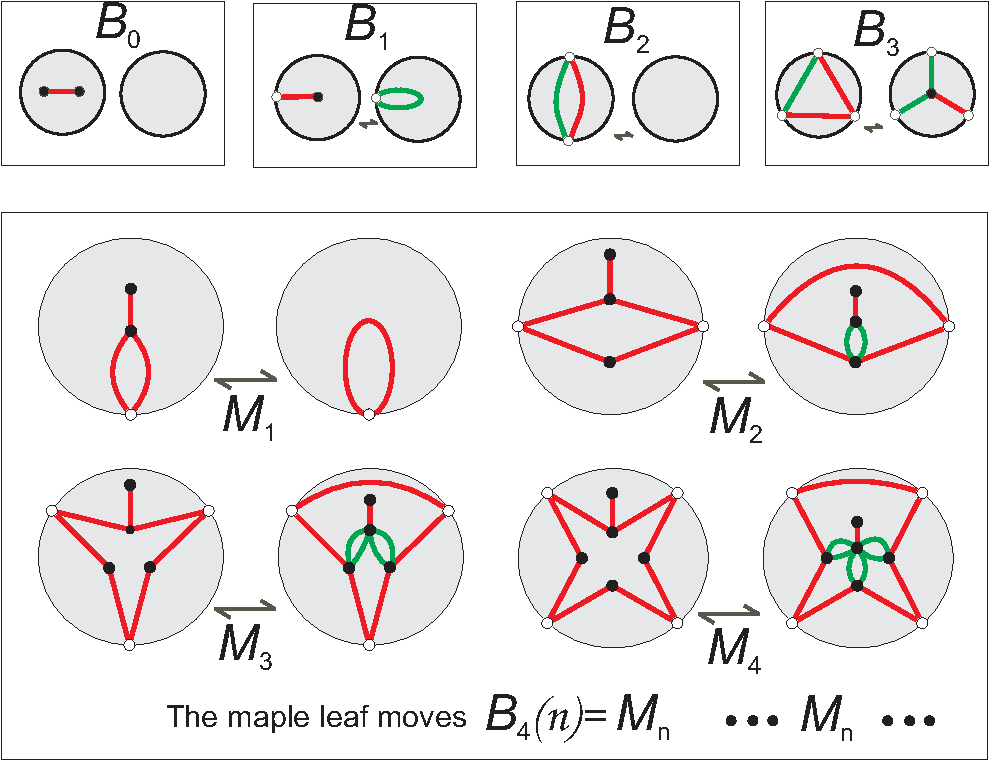
\includegraphics[width=10cm]{E.figsbw2/blinkcalculusoncoins.pdf}
   \end{center}
   \vspace{-0.7cm}
   \caption{Blink formal calculus by local coins replacements}
   \label{fig:blinkCalculusOnCoins}
\end{figure}
Some explanation on Figure \ref{fig:blinkCalculusOnCoins} is in
order. The portion of the blinks which are altered is depicted in
an open disk named a {\em coin}. The interior of the coins modifies
precisely as indicated. The vertices interior to a coin are
displayed as small black circles. The intersection of the blink with
the complement of the coin is a subset of vertices, the {\em
attachment} vertices displayed as small white circles. In this way a
point in the interior of an edge of the blink is either inside or
else outside the coin. We allow arbitrary identifications in the
attachment vertices via deformations of the coins so as to preserve
their interiors (as long as they preserve planarity).

In ${\cal B}$ there are four simple moves twins: $B_0$, $B_1$,
$B_2$, $B_3$, and an infinite family $B_4(1)={M}_1$,\
$B_4(2)={M}_2$,\ $B_4(3)={M}_3$, $\ldots$, named the {\em maple leaf
moves}, $B_4(n) = {M}_n$. By an abuse of notation, each move
$B_i,$ ($i=0,1,2,3$) or $M_n,$ $n \in \mathbb{N}$, denotes either the move
depicted in Figure \ref{fig:blinkCalculusOnCoins} or its red/green
twin.


The maple leaf move $M_n$ is the manifestation in the blink of the
move $\mu'_n$ on BFLs treated in the subsection which follows the
next one. Move $\mu'_n$ will replace move $\alpha_n$ which
is another name for move $K_4(n)$ shown on Figure~\ref{fig:BFLcalculusK1}.
We stress the point that the set of axioms in the above formal ${\cal
L}$-calculus is a minimal one. For instance, we anticipate the fact
that a move obtained from a move in $\B$ by taking planar duals of
the blinks is a consequence of $\B$.

\bigskip \bigskip \centerline{\bf \large In BFLs, $\mu_n$ is equivalent to $\alpha_n$} \bigskip

We now show that the $\alpha_n$ axiom on BFLs can be replaced by a
new axiom: $\mu_n$. This is useful because the number of crossings
involved in $\mu_n$ is linear on $n$ while in $\alpha_n$ is
quadratic. The axiom $\mu_1$ is defined to coincide with $\alpha_1$.
For $n >1$, $\mu_n$ is defined by Figure \ref{fig:mun}.

\begin{figure}[htp]
   \begin{center}
      \leavevmode
      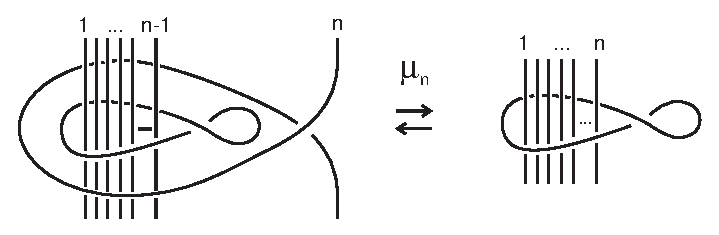
\includegraphics[width=10cm]{A.figs/mun.eps}
   \end{center}
   \vspace{-0.7cm}
   \caption{Definition of $\mu_n$, $n \geq 2$.}
   \label{fig:mun}
\end{figure}

\begin{lemma} \label {lem:heartSmoothing}  The heart-shape smoothing
move depicted below is obtained regular isotopies, and a single
ribbon move.
\begin{center}
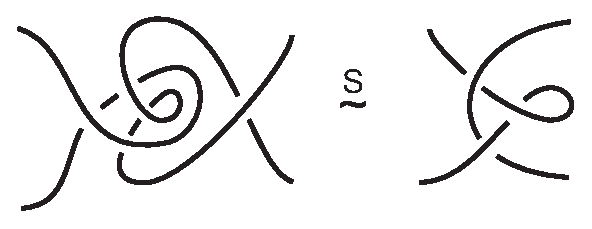
\includegraphics[width=6cm]{A.figs/heartsmoothing.eps}
\end{center}
\end{lemma}
\begin{proof}Follow the proof in the figure below. The ribbon move
is used in the second configuration to prepare for the application
of Whitney�s trick. After this is done we obtain the third
configuration. All other moves are regular isotopies.
\begin{center}
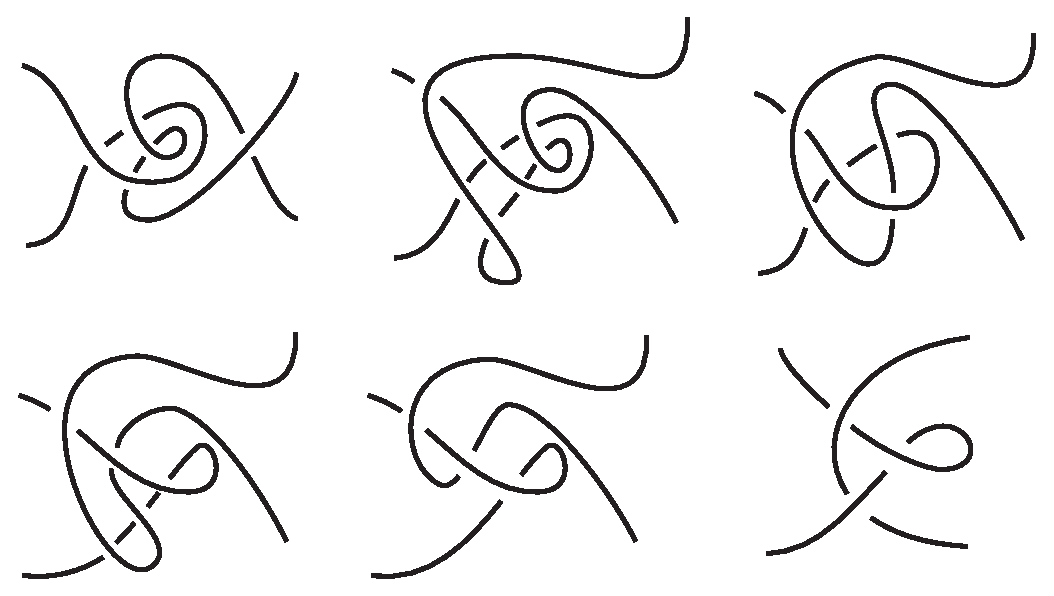
\includegraphics[width=12cm]{A.figs/heartsmoothingproof.eps}
\end{center}
\vspace{-0.8cm}
\end{proof}

\begin{lemma} The move $\mu_n$ does not change the induced space.
\end{lemma}
\begin{proof} The proof is done for a class of moves that
generalizes $\mu_n$, depicted in Fig. \ref{fig:muNproof}.
\begin{figure}[htp]
   \begin{center}
      \leavevmode
      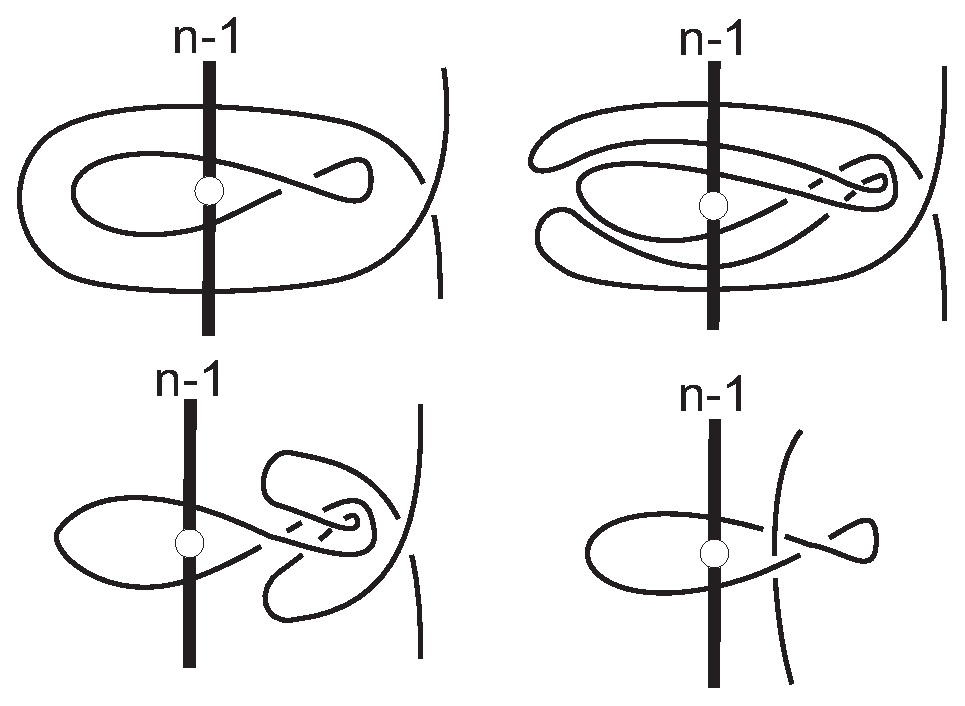
\includegraphics[width=9cm]{A.figs/munproof.eps}
   \end{center}
   \vspace{-0.7cm}
   \caption{Moves that generalize $\mu_n$.}
   \label{fig:muNproof}
\end{figure}
The white circle separating the cable of $n-1$ parallel strands
means that the $2(n-1)$ individual strands in its boundary are
paired arbitrarily (maintaining planarity, of course). The precise
undercrossings and overcrossings of the individual strands in the
cable are also arbitrary and are left undisplayed: we indicate this
by a real crossing between the thick line and the thinner ones. The
first passage from the first to the second configuration, is a Kirby
handle slide (page 122 of \cite{KauffmanAndLins1994}) obtained by
doubling the $\infty$-shaped component and performing the connected
sum at the external encircling component. Note that (irrespectively
of the individual crossings not shown) the third configuration is
reachable from the second by Reidemeister moves of type II because
consecutive crossings along the individual
strands inside the cable are both over or both under. The third
passage is a consequence of the heart-smoothing move of Lemma
\ref{lem:heartSmoothing}
\end{proof}

\begin{lemma} $\mu_1, \mu_2, \mu_3, \ldots \Rightarrow \alpha_n$ for all $n\geq 1$. In words:
if you have the infinite sequence of moves $\mu_1,\mu_2,\ldots$ then
you can reproduce $\alpha_n$ for any $n \geq 1$.
\end{lemma}
\begin{proof} By induction on $n$. It is obvious that we
have $\alpha_1$ from $\mu_1, \mu_2, \mu_3, \ldots $ once, by
definition, $\alpha_1 = \mu_1$. Suppose we have how to reproduce
$\alpha_i$ from $\mu_1,\mu_2,\ldots$ for all $i < n$. Then, for $n$,
as can be seen on the Figure below, we can apply the induction
hypothesis on the internal $n-1$ strands of the curl and then apply
the $\mu_n$, thus obtaining $\alpha_n$.
\begin{center}
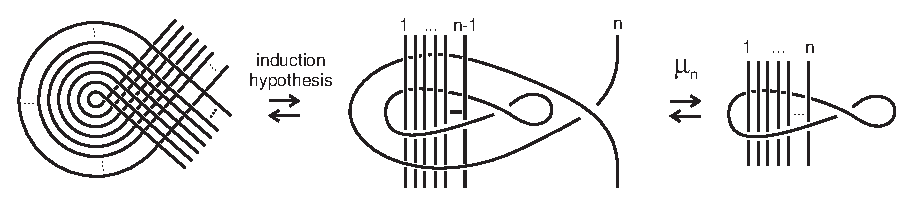
\includegraphics[width=12cm]{A.figs/munimpliesalphanproof.eps}
\end{center}
\end{proof}

\bigskip \bigskip \centerline{\large \bf In BFLs,  $\mu_n$ is equivalent to $\mu'_n$} \bigskip

By replacing $\alpha_n$ with $\mu_n$ we have simplified our axioms
in the sense that $\mu_n$ has fewer crossings than $\alpha_n$. But,
before translating our axiom system on blackboard framed links to
the blink language, we define the move $\mu'_n$ that is equivalent to
$\mu_n$ but has a ``better'' translation to blinks. The axiom
$\mu'_1$ is equal to $\mu_1$. For $n \geq 2$, $\mu'_n$ is defined by
the schema on Figure \ref{fig:MuNLinha}.

\begin{figure}[htp]
   \begin{center}
      \leavevmode
      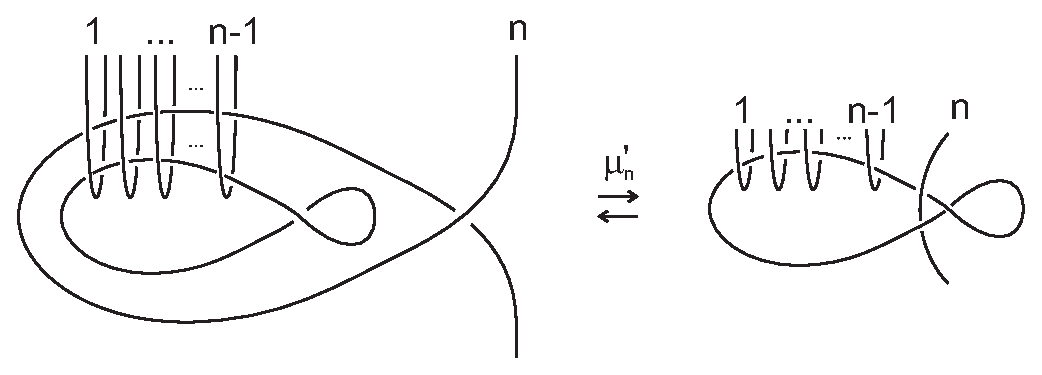
\includegraphics[width=10cm]{A.figs/munlinha.eps}
   \end{center}
   \vspace{-0.7cm}
   \caption{The axiom $\mu'_n$ ($n \geq 2$) : ``better'' blink translation than $\mu_n$}
   \label{fig:MuNLinha}
\end{figure}

\newpage

\begin{proposition} (Regular isotopy and $\mu'_n$) $\Rightarrow
\mu_n,\,\,\,$ for $n\geq 1$.
\end{proposition}
\begin{proof}
For $n=1$ it is obvious because $\mu_1=\mu_1'$. The figure below
shows the proof for $n=2$. Beginning with the right side of $\mu_2$
we apply regular isotopy ({\it i.e} moves $K_2$ and $K_3$) until we
get to a pattern where $\mu_2'$ can be applied (the second pattern
on the second line). We apply it and then use again regular isotopy
to get to the pattern of the left side of the $\mu_2$ axiom. As all
these transformations are both ways, we have proved the case for
$n=2$. The proof for $n>2$ is analogous to the $n=2$ case and will
not be shown.
\begin{center}
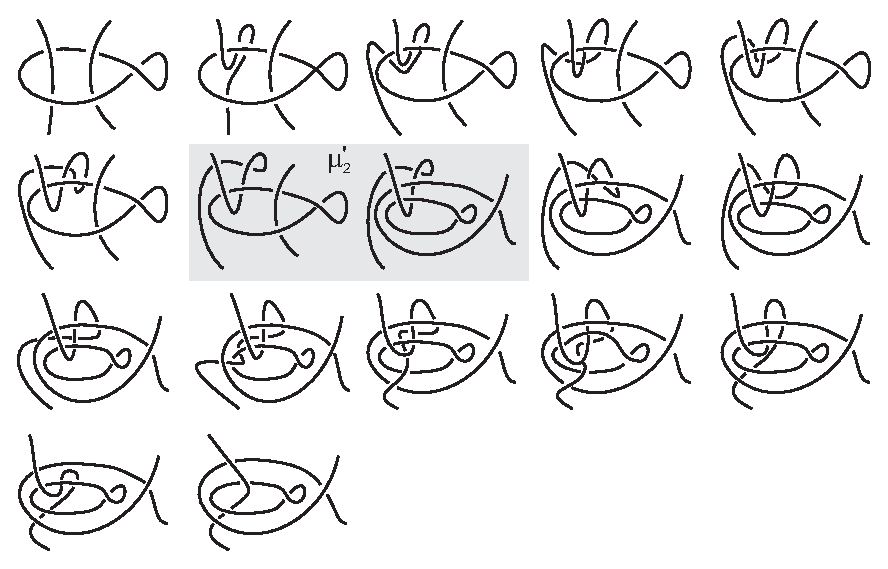
\includegraphics[width=13cm]{A.figs/munlinhaimpliesmunproof.eps}
\end{center}
\vspace{-1cm}
\end{proof}

\bigskip \centerline{\bf \textsc{Translation of Blackboard Framed Link Calculus to Blink Calculus}} \bigskip

The translation from $\mathcal{K}$ into $\mathcal{B}$ is depicted 
in Figure~\ref{fig:translationBFLCalculusToBlinkCalculus}.

\begin{figure}[htp]

\begin{center}
\leavevmode
\begin{footnotesize}
\begin{tabular}{|c|c|} \hline
\rule{0cm}{2.7cm}
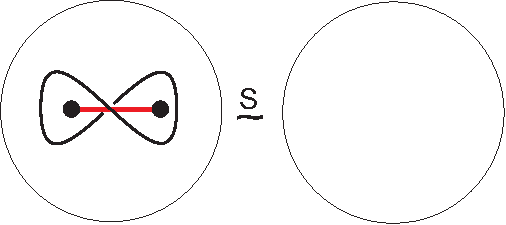
\includegraphics[width=5cm]{E.figsbw2/translationk0.pdf} &
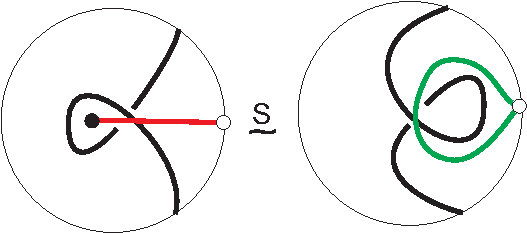
\includegraphics[width=5cm]{E.figsbw2/translationribbonmove.pdf} \\
Translation of $K_0$ into $B_0$ &
Translation of the ribbon move $K_1$ into $B_1$ \\ \hline
\rule{0cm}{2.7cm}
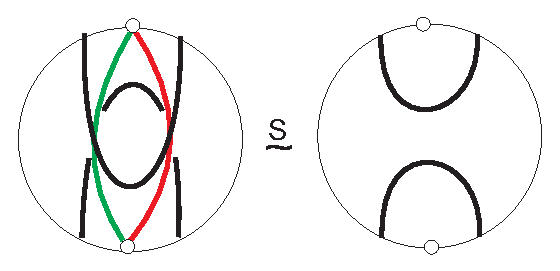
\includegraphics[width=5cm]{A.figs/translationk2.eps} &
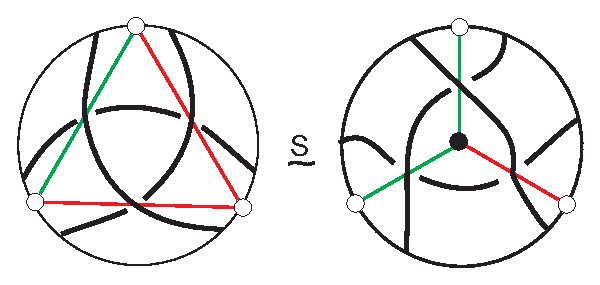
\includegraphics[width=5cm]{A.figs/translationk3.eps} \\
Translation of $K_2$ into $B_2$ &
Translation of $K_3$ into $B_3$ \\ \hline
\multicolumn{2}{|c|}{
      \rule{0cm}{7.4cm} 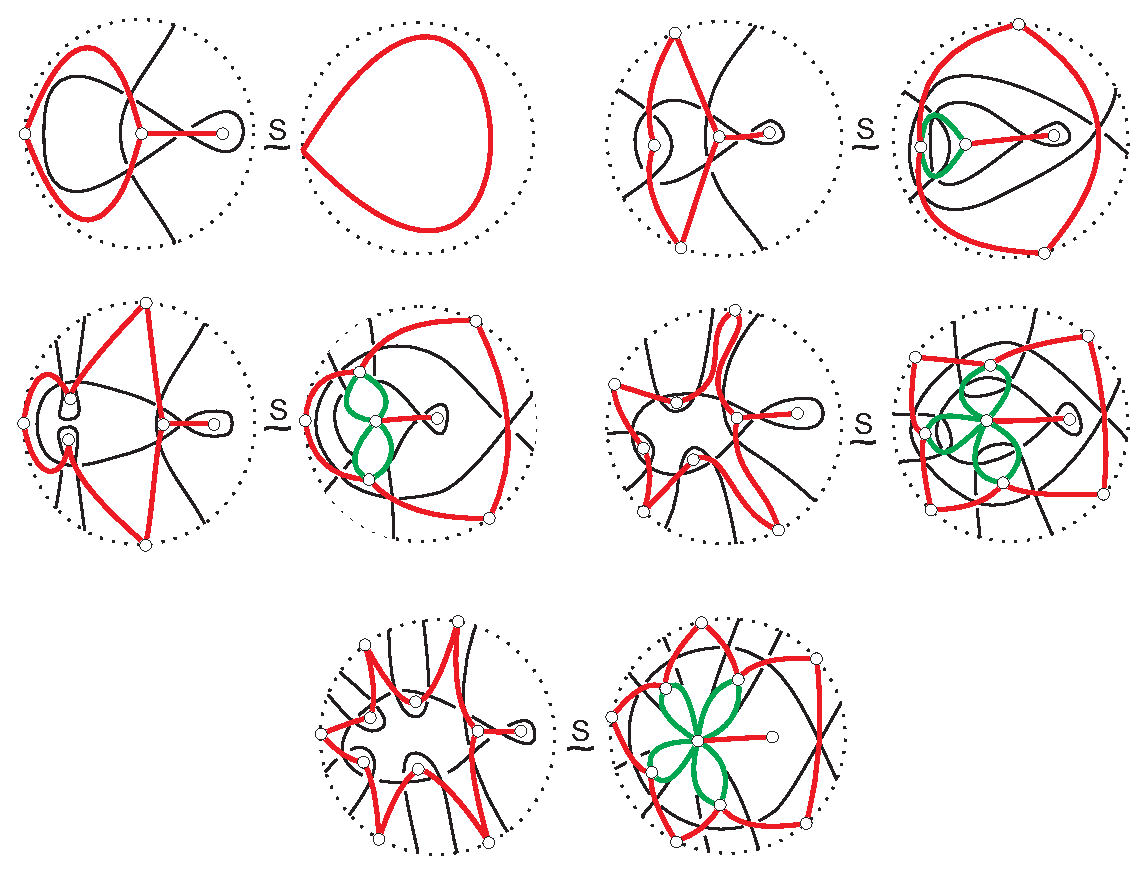
\includegraphics[width=9cm]{A.figs/munlinhatranslation2.eps}
} \\
\multicolumn{2}{|c|}{
      Translation of $\mu'_1, \ldots, \mu'_5, \ldots$,
   into $M_1, \ldots, M_5, \ldots$
} \\ \hline
\end{tabular}
\end{footnotesize}
\end{center}
   \vspace{-0.5cm}
   \caption{Translation of BFL calculus to blink calculus}
   \label{fig:translationBFLCalculusToBlinkCalculus}
\end{figure}


\begin{proof}(of Theorem \ref{theo:blinkCalculus}.) The proof is a direct translation
of the moves $K_0, \ldots, K_3$ and $\mu'(1),\ldots \mu'_n,\ldots,$
into the moves $B_0, \ldots B_3$, and $M_1, \ldots K_n, \ldots$
\end{proof}

\subsection{g-blinks}
\label{sec:gblinks}

Let $B$ be a blink. We now describe a procedure to define, from $B$,
a 4-regular graph $G_B$ named a \hbox{\it g-blink}. This procedure is
called \textsc{Blink2GBlink} and associates to any blink
(topological object) a unique g-blink (combinatorial object). Let
$u$ be a vertex of $B$ and $e_0,\ldots,e_{\delta_u-1}$ be the edges
incident to $u$ ordered in clockwise direction ($e_0$ may be any
edge). For each edge $e_i$ with $i \in \{0,\ldots,\delta_u-1\}$ we
define two vertices in $G_B$: one labeled $(u,e_i,2i)$ positioned
close to $e_i$ but before it in clockwise direction; the other is
labeled $(u,e_i,2i+1)$ positioned close to $e_i$ but after it in
clockwise direction (see Figure \ref{fig:gblinkFromBlinkElements}A).
If $(u,e,2j)$ and $(u,e,2j+1)$ are vertices of $G_B$ then they are
the ends of a {\it face-edge} of $G_B$ (Figure
\ref{fig:gblinkFromBlinkElements}B). If $(u,e,2j+1)$ and $(u,f,2j+2
\hbox{ \rm mod } 2\delta_u)$ are vertices in $G_B$ then they are the
ends of a {\it angle-edge} in $G_B$ (Figure
\ref{fig:gblinkFromBlinkElements}B). If $(u,e,j)$ and $(v,e,k)$ are
vertices in $G_B$ and the parity of $j$ is different from the parity
of $k$ then they are the ends of a {\it vertex-edge} of $G_B$
(Figure \ref{fig:gblinkFromBlinkElements}C). If $(u,e,j)$ and
$(v,e,k)$ are vertices in $G_B$ and the parity of $j$ is equal to
the parity of $k$ then they are the ends of a {\em zigzag-edge} of
$G_B$ (Figure \ref{fig:gblinkFromBlinkElements}D).
\begin{figure}[htp]
   \begin{center}
      \leavevmode
      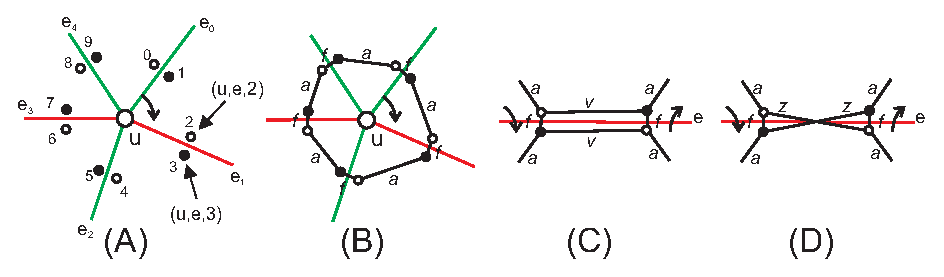
\includegraphics{A.figs/gblinkfromblinkelements.eps}\\
   \end{center}
   \vspace{-0.7cm}
  \caption{Elements on the definition of a g-blink from a blink}
  \label{fig:gblinkFromBlinkElements}
\end{figure}

We define a bipartition $V_0$ and $V_1$ of the vertices of $G_B$
like this: a vertex $v$ labeled with $(\_\, , \_\, ,2j)$, for some integer
$j$, is said to be a {\em parity zero vertex} and it is in $V_0$; a
vertex $v$ labeled with $(\_\, ,\_\, ,2j+1)$, for some integer $j$, is said
to be a {\em parity one vertex} and it is in $V_1$. On the example
of Figure \ref{fig:Blink2GBlinkExample} $V_0$ are the white vertices
and $V_1$ are the black vertices.

If $B$ has $n$ edges, then $G_B$ has $4n$ vertices and $8n$ edges.
Each vertex of $G_B$ has degree 4 and is incident to a face-edge, an
angle-edge, a vertex-edge and a zigzag-edge. If $v$ is a vertex in
$G_B$ we denote by ${\rm adj}_v(v)$, ${\rm adj}_f(v)$, ${\rm
adj}_a(v)$ and ${\rm adj}_z(v)$ the vertices adjacent to $v$ by
vertex-edge, face-edge, angle-edge and zigzag-edge respectively.

\begin{figure}[htp]
   \begin{center}
      \leavevmode
      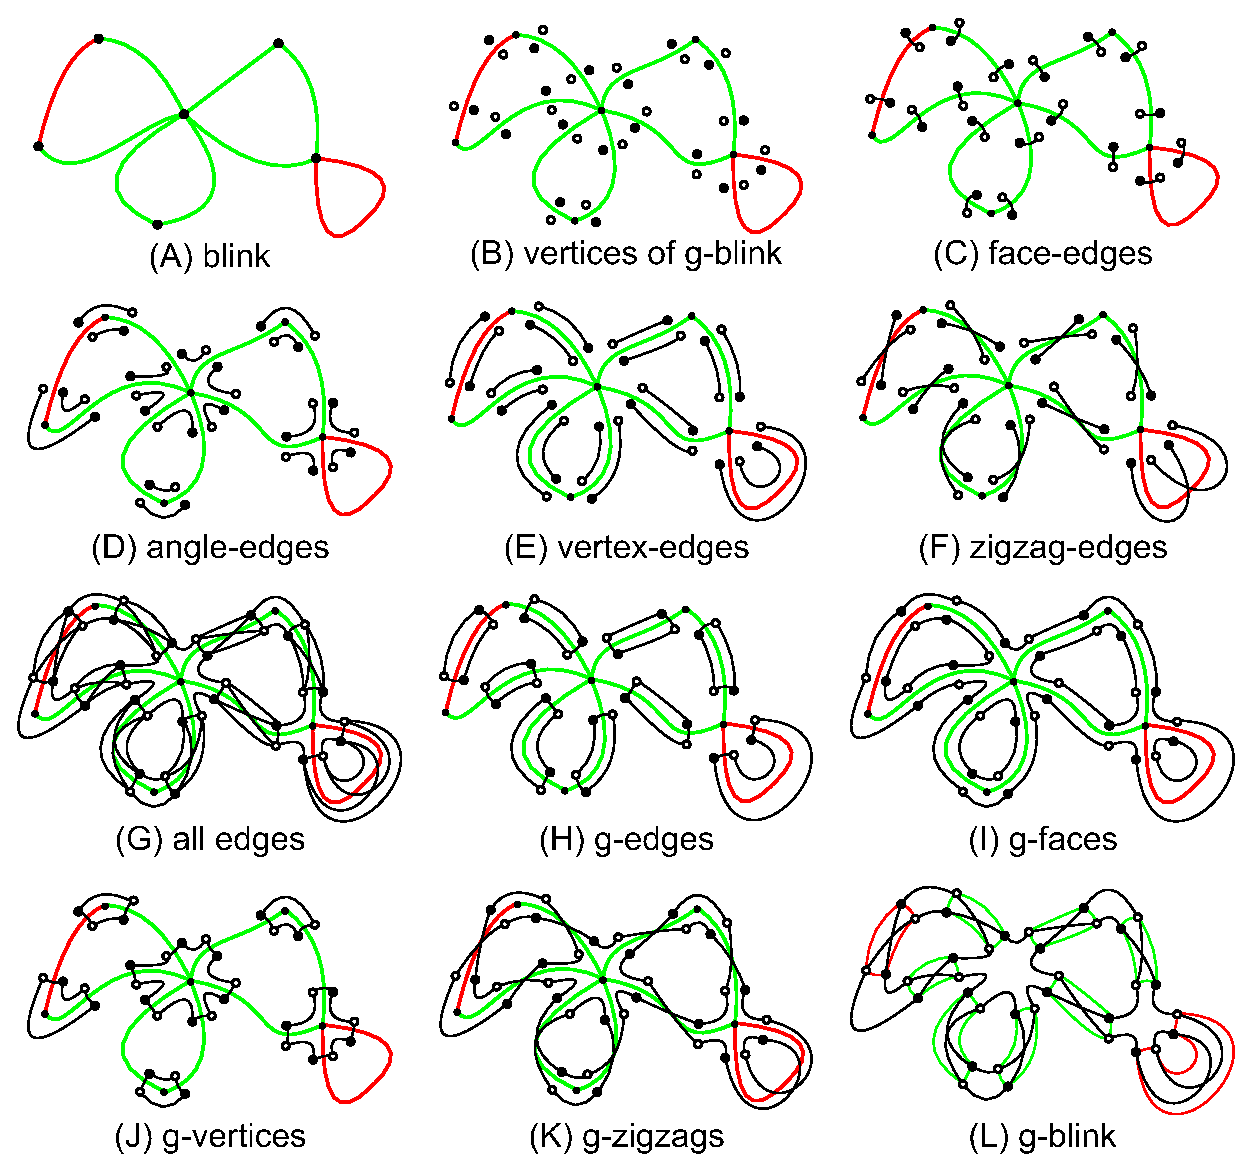
\includegraphics[width=14cm]{A.figs/blink2gblinkexample.eps}\\
   \end{center}
   \vspace{-0.7cm}
  \caption{Blink, g-blink and attributes: an example}
  \label{fig:Blink2GBlinkExample}
\end{figure}

A {\it g-edge} is a polygon on a g-blink whose edges alternate
between face-edges and vertex-edges (Figure
\ref{fig:Blink2GBlinkExample}H). A g-edge has always 4 edges and 4
vertices and is associated to an edge on a blink (note that the
vertices of a g-edge are of the form $(\_\, ,e,\_)$). If the
corresponding blink edge of a g-edge is red then this g-edge is also
red. If the corresponding blink edge of a g-edge is green then this
g-edge is also green. A {\it g-face} of a g-blink is any polygon
with vertex-edge alternated with angle-edge (Figure
\ref{fig:Blink2GBlinkExample}I). Each of these polygons corresponds
to a face of the blink. A {\it g-vertex} of a g-blink is any polygon
with face-edge alternated with angle-edge (Figure
\ref{fig:Blink2GBlinkExample}J). Each of these polygons corresponds
to a vertex of the blink. A {\it g-zigzag} of a g-blink is any
polygon with angle-edge alternated with zigzag-edge (Figure
\ref{fig:Blink2GBlinkExample}K). Each of these polygons corresponds
to a component on the blackboard framed link associated with the
blink.

Now, using the notation defined above, we state a definition for
{\it g-blink}. A {\it g-blink} is a graph that satisfies the
following six conditions:

\vspace{-0.1cm}

\begin{enumerate}
% locally change parident and parskip
%\setstretch{1.5}
% parskip
\setlength{\parskip}{-2pt} \sl


\item[(1)] Its vertices are partitioned in $V_0$ and $V_1$ (white and black
vertices of Figures \ref{fig:gblinkFromBlinkElements} and
\ref{fig:Blink2GBlinkExample});

\item[(2)] vertices in $V_0$ are adjacent by face-edge, vertex-edge and
angle-edge to vertices in $V_1$ and by zigzag-edges to vertices in
$V_0$; vertices in $V_1$ are adjacent by face-edge, vertex-edge and
angle-edge to vertices in $V_0$ and by zigzag-edges to vertices in
$V_1$;

\item[(3)] each vertex is incident to exactly one face-edge, one
vertex-edge, one angle-edge and one zigzag-edge;

\item[(4)] each polygon of alternating face-edge and vertex-edge has
4 edges (is a g-edge) and is assigned color red or green
(see the g-edges on Figure~\ref{fig:Blink2GBlinkExample}L) or,
equivalently, a pair of zigzag edges of the same g-edge is labeled
one edge as {\it overcrossing} and the other edge as {\it
undercrossing};

\item[(5)] the zigzag-edges are the diagonals of the g-edges connecting
the vertices with the same parity. Observe that this implies that
zigzag-edges are redundant when we know the g-edges. They may be
omitted when presenting a g-blink and calculated or shown when
needed. For example Figure~\ref{fig:Blink2GBlinkExample}L can be
easily restored from Figure~\ref{fig:gBlinkWithoutZigzags};

\item[(6)] the 3-regular graph obtained by not considering the zigzag
edges is a planar graph (see Figure \ref{fig:gBlinkWithoutZigzags}).

\end{enumerate}


\begin{figure}[htp]
   \begin{center}
      \leavevmode
      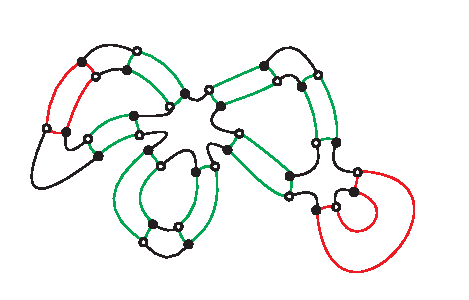
\includegraphics[width=6cm]{A.figs/gblinkwithoutzigzags.eps}\\
   \end{center}
   \vspace{-0.7cm}
  \caption{g-blink of Figure \ref{fig:Blink2GBlinkExample}L without zigzag-edges: a planar graph}
  \label{fig:gBlinkWithoutZigzags}
\end{figure}


It is important to note that a g-blink is a combinatorial object,
although, to visualize the connection with blinks, we show drawings
of g-blinks where edges are curves and vertices are points. These
drawings are just to help visualization. The g-blink relevant
information is combinatorial: a set of vertices, the neighbor of
each vertex by each type of edge, the parity of the vertices and the
color of the g-edges.

Note that the definition of g-blinks is independent of blinks. As we
saw, it is a 4-regular graph with some additional structures and
constraints. Now, with this observation in mind, consider the
situation shown on Figure~\ref{fig:DifferentBlinksSameGBlink}. The
blinks of Figure~\ref{fig:DifferentBlinksSameGBlink}A and
Figure~\ref{fig:DifferentBlinksSameGBlink}D are different in the
strict sense (their plane graphs are different) but are
different\footnote{When referring to blinks, this looser sense
concept of ``difference'' is the one we adopted as our convention on
Section \ref{sec:BFL2Blinks}. We could just say the blink of
Figure~\ref{fig:DifferentBlinksSameGBlink}A and the blink of
Figure~\ref{fig:DifferentBlinksSameGBlink}D are different.} in a
looser sense also: there is no plane isotopy between these two
blinks (we would have to tear the red loop on
Figure~\ref{fig:DifferentBlinksSameGBlink}A). On the other hand,
their g-blinks are the same as can be seen on
Figure~\ref{fig:DifferentBlinksSameGBlink}C and
Figure~\ref{fig:DifferentBlinksSameGBlink}F (remember that the edges
on g-blinks presented as drawings are important only to define who
is the neighbor of who, their curve shape is not important).

\begin{figure}[htp]
   \begin{center}
      \leavevmode
      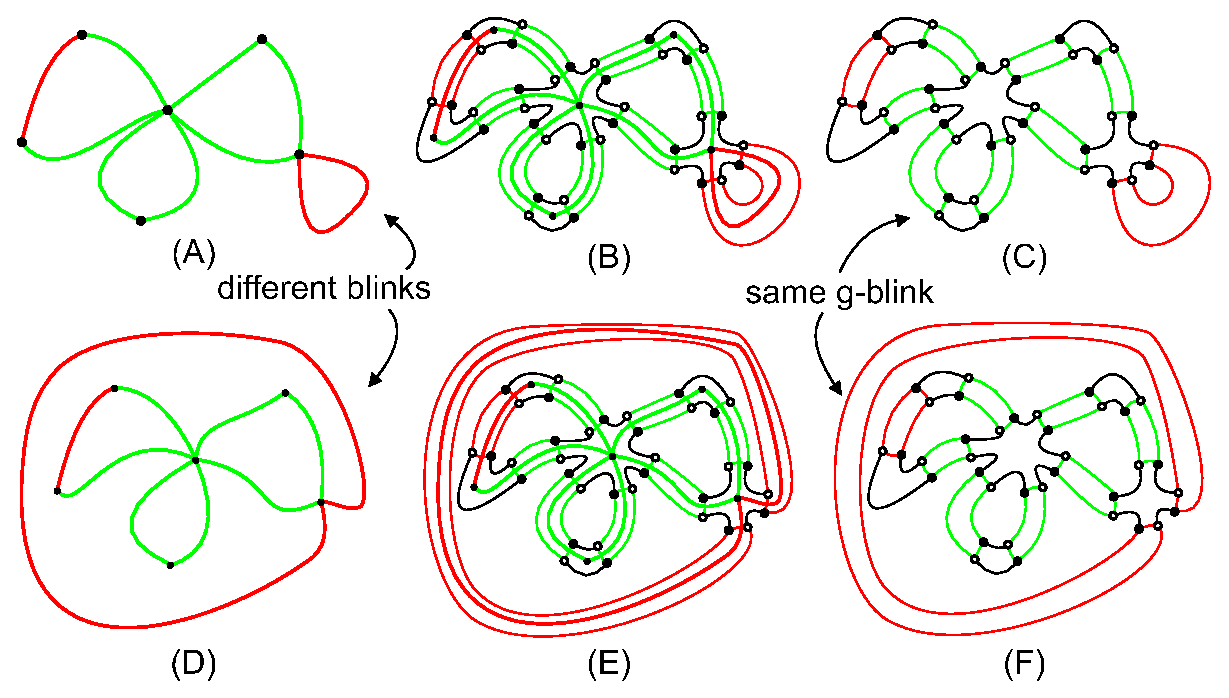
\includegraphics[width=12cm]{A.figs/differentblinkssamegblink.eps}\\
   \end{center}
   \vspace{-0.7cm}
  \caption{Different blinks with the same g-blink}
  \label{fig:DifferentBlinksSameGBlink}
\end{figure}

To obtain a blink from a g-blink we must first embed (forgetting
zigzag-edges) the g-blink on a plane respecting the convention we
used on the procedure \textsc{Blink2GBlink}: the orientation of all
g-vertices induced by orienting the face-edges from white (parity 0
vertex) to black (parity 1 vertex) is always clockwise. Let's name
this convention as {\em convention} $\circlearrowright$. The
embedding part is always possible once a g-blink without
zigzag-edges is a planar graph. It is always possible to
satisfy convention $\circlearrowright$. For example, if all
\hbox{g-vertices} are counterclockwise we may reflect horizontally or
vertically all the embedding correcting the situation. If all
g-vertices are correct except for the external g-vertex (which is
the external face in this case) then we may redraw the curve of an
external angle-edge making it go around all the embedding (see edge
$e$ for an example of this on Figure~\ref{fig:dualGBlinksInduceSameSpace}). If a
blink $B$ is obtained from a g-blink $G$ then we say that $G$
induces $B$.

What are the blinks induced by a g-blink? We must answer this to
continue. Name $A$ the blink of
Figure~\ref{fig:DifferentBlinksSameGBlink}A and $B$ the blink on
Figure~\ref{fig:DifferentBlinksSameGBlink}D. We know there is no
plane isotopy between $A$ and $B$. But $A$ and $B$ are both
obtainable from the same g-blink as
Figure~\ref{fig:DifferentBlinksSameGBlink} shows. How could we
connect $A$ and $B$? The answer is shown on
Figure~\ref{fig:SphereIsotopy}. On the sphere $\mathbb{S}^2$ there is an
isotopy between $A$ and $B$. One can check that blinks obtainable
from a g-blink are blinks that when embedded on a sphere (draw it on
the plane and then use stereographic projection to get this
embedding) may be transformed one into the other by an isotopy of
the sphere.
\begin{figure}[htp]
   \begin{center}
      \leavevmode
      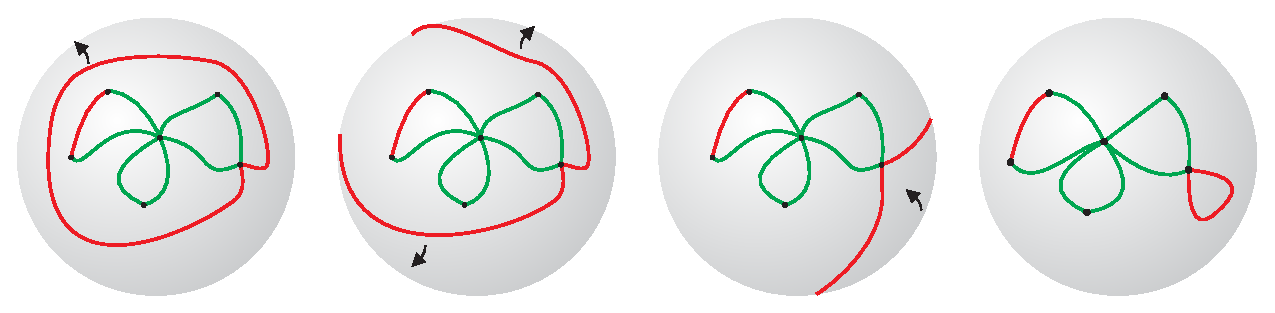
\includegraphics[width=11cm]{A.figs/sphereisotopy.eps}
   \end{center}
   \vspace{-0.7cm}
   \caption{Isotopy on the sphere $\mathbb{S}^2$}
   \label{fig:SphereIsotopy}
\end{figure}

Do the blinks obtainable from a g-blink induce the same space? Once
we are, at the end, interested in spaces, g-blink would not be a
useful object if its blinks induced different spaces. The answer
is yes. All blinks of a g-blink induce the same space. The reason is
the \hbox{Blink Jumping Rope Lemma \ref{lem:BlinkJumpingRopeLemma}}.
Note how this Lemma is exactly what is needed to prove that the
blinks of Figure~\ref{fig:DifferentBlinksSameGBlink}A and
Figure~\ref{fig:DifferentBlinksSameGBlink}D induce the same space.

\pagebreak

\begin{lemma}[Blink Jumping Rope Lemma] \label{lem:BlinkJumpingRopeLemma}
The (meta-)blinks shown below induce the same space.
    \begin{center}
        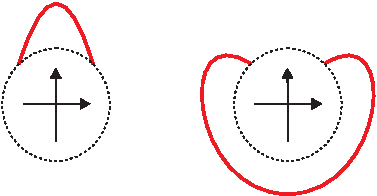
\includegraphics[width=5cm]{E.figsbw2/blinkjumpingropelemma.pdf}
    \end{center}
\end{lemma}
\begin{proof} Follow the figure below. First we show the BFL
associated with the left blink (the crossing correspondent to red
edge). Then we apply the Jumping Rope Lemma
\ref{lem:jumpingRopeLemma} for BFLs and regular isotopy to get to
our target blink. As our moves preserve the space, we have the
result.
    \begin{center}
        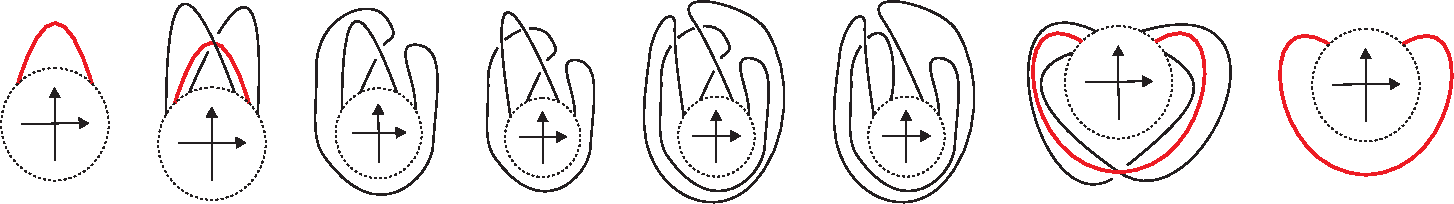
\includegraphics[width=14cm]{E.figsbw2/blinkjumpingropelemmaproof.pdf}
    \end{center}
\vspace{0.1cm}
\end{proof}

With this last result we now define the {\it space of a g-blink} as
the space induced by any blink induced by the g-blink. As we saw,
this space is unique. Observe that the blinks induced by a g-blink
are divided into $|F|$ plane isotopy classes, where $F$ is the set
of g-faces of the g-blink. For each g-face $f \in F$ there is a
blink which has the face corresponding to $f$ as its external face.
So, not considering symmetries that may occur, each g-blink
corresponds to $|F|$ distinct blinks.

Although our initial motivation was to work with blinks, in practice
we did this indirectly through g-blinks. It turned out that this was more
adequate once g-blinks are simpler (i.e. to encode a single blink we would
have to have the current g-blink information plus an extra one: which
g-face is the external one), more expressive (for instance, one g-blink actually
encodes $|F|$ blinks that induce the same space) and we could prove a
set of g-blink interesting properties that enabled us to do the
experiments we wanted (for example, find all distinct spaces that had a small
blink/BFL/g-blink presentation).

Before ending this section, one last observation: note that a single g-blink
also encodes $|F|$ BFLs: the ones obtained from the $|F|$ blinks by the
\textsc{Blink2BFL} procedure. So we may see a g-blink through $|F|$ blink
views and through $|F|$ BFL views.

\subsection{Homology group from g-blink}
\label{sec:homologyGroup}

The homology group is a topological invariant obtained from the
abelianization of the fundamental group. It is easy to obtain a
presentation of the fundamental group from a blackboard framed link.
However, the problem of deciding if two presentations of a group are
isomorphic is an undecidable problem. This does not occur with the
homology group. It is presented as a pair $(b,t)$, where $b$ is the
{\it Betti number} and $t=(t_1,\ldots,t_p)$ is a sequence with
$p\geq 0$. Each $t_i$ in $t$ is called the $i$-th torsion
coefficient. This sequence also satisfies: $t_1 \geq 2$, if $p > 0$
and $t_i$ divides $t_{i+1}$ for $i<p$. The homology group $(b,t)$
may be obtained from the Smith Normal Form of the linking matrix
of a BFL (see \cite{nemhauser1988integer} for definition and how to obtain
this normal form). This is so because the linking matrix is a relation matrix for
the homology group. The number of zeros in this diagonal
is the Betti number $b$ and appear all at the end. Throw away the
entries equal to 1. The torsion coefficients $t=(t_1,\ldots,t_p)$
are the other entries on the diagonal. The remainder of this section
shows how to calculate the linking matrix from a g-blink.

Let $Z = \{ z_1, \ldots, z_k \}$ be the set of g-zigzags of the g-blink
$G$. So every $z$ in $Z$ is a polygon with alternating zigzag-edges
and angle-edges. We want to define a matrix $N$ of dimension $k
\times k$. First we orient each g-zigzag $z$ in $Z$. This can be
done by mounting a list $v_1, \ldots, v_m$ of the vertices of z such
that $v_i$ is adjacent to $v_{i+1}$ by an edge in $z$, $v_m$ is
adjacent to $v_1$ by an edge in $z$ and the orientation of the edges
in $z$ is defined by the way its end vertices appear in the list: the
edge of $z$ between $v_i$ and $v_{i+1}$ is oriented from $v_i$ to
$v_{i+1}$ for $1\leq i \leq m-1$ and the edge of $z$ whose ends are
$v_1$ and $v_m$ is oriented from $v_m$ to $v_1$. Initialize all
entries of $N$ with zero. For each g-edge $a$, let $u$ and $v$ be
vertices in $a$ such that: $u$ has parity zero (in $V_0$ or white);
$v$ has parity one (in $V_1$ or black); $z_i$ is the g-zigzag
incident to $u$; $z_j$ is the g-zigzag incident to $v$; the
zigzag-edge in $z_i$ incident to $u$ and $u'$ is oriented this way
from $u$ to $u'$; the zigzag-edge in $z_j$ incident to $v$ and $v'$
is oriented this way from $v$ to $v'$. Aligning each g-edge $a$ to
this standard leads to one of the situation shown in
Figure~\ref{fig:linkingMatrix} where the sign $s_a$ of $a$ is also
shown. If $a$ is green and $u$ is adjacent to $v$ by a face-edge
then $s_a=+1$ (Figure~\ref{fig:linkingMatrix}A). If $a$ is red and
$u$ is adjacent to $v$ by a face-edge then $s_a=-1$
(Figure~\ref{fig:linkingMatrix}B). If $a$ is green and $u$ is
adjacent to $v$ by a vertex-edge then $s_a=-1$
(Figure~\ref{fig:linkingMatrix}C). If $a$ is red and $u$ is adjacent
to $v$ by a vertex-edge then $s_a=+1$
(Figure~\ref{fig:linkingMatrix}D).
\begin{figure}[htp]
   \begin{center}
      \leavevmode
      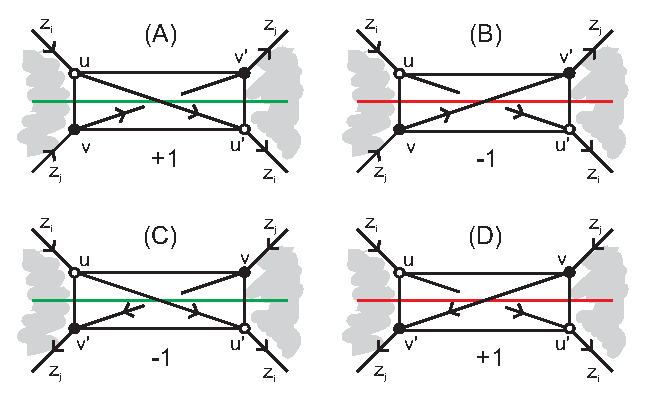
\includegraphics[width=8cm]{A.figs/linkingmatrix.eps}
   \end{center}
   \vspace{-0.7cm}
   \caption{ Signs of a g-edge $a$ for the linking matrix}
   \label{fig:linkingMatrix}
\end{figure}

Knowing the sign of $a$ we update $N$ by $$N_{i,j} \leftarrow
N_{i,j} + s_a$$ and, if $i \neq j$, we also do $$N_{j,i} \leftarrow
N_{j,i} + s_a.$$ Note that $N$ is symmetric. Once $N$ is defined, to
calculate the homology group is to calculate the Smith Normal Form
of $N$ and then collect the pair $(b,t)$ as was already described
above.

\subsection{Quantum invariant from g-blink}
\label{sec:quantumInvariant}

 In this section we show how to calculate
the Witten-Reshetikhin-Turaev quantum invariant for a space from a
g-blink inducing it. This calculation is a translation to g-blinks
of the one showed on \cite{Lins1995} that operates over blackboard
framed links. For further details for this invariant see
\cite{KauffmanAndLins1994}.


The Witten-Reshetikhin-Turaev invariant for a space $M$ is a
function ${\rm wrt}_M:\{3,4,\ldots\} \rightarrow \mathbb{C}$. This function
maps every integer $i\geq 3$ into a complex number ${\rm wrt_M}(i)
\in \mathbb{C}.$ If two spaces $A$ and $B$ satisfy ${\rm wrt}_{A}(i) \neq
{\rm wrt}_{B}(i)$ for some $i$ then $A$ and $B$ are different
spaces.

Let $M$ be a space and $r \geq 3$ an integer for which we want to
obtain ${\rm wrt}_M(r).$ Let ${\cal I} = \{0,1,\ldots,r-2\}$. Let
$A$ be a $(4r)$-primitive-root of 1. For $n \in {\cal I}$ define
$$\Delta_n = (-1)^n \, \frac{A^{2n+2}-A^{-2n-2}}{A^{2}-A^{-2}},$$
$${[n]} = \frac{A^{2n}-A^{-2n}}{A^2-A^{-2}} =
(-1)^{n-1}{\Delta_{n-1}}\,.$$ Define $q = A^2$ and, for reasons
inherited from physics, call $[n]$ by {\em q-deformed quantum
integer } and
$$ [n]! = \prod_{1\leq m \leq n}{[m]}$$ by {\em q-deformed
quantum factorial.} Note that although $A$ is a complex number,
$\Delta_n$ and $[n]$ are real numbers. Three numbers $a,b,c \in {\cal
I}$ are said to be an {\em $r$-admissible triple} if $a+b+c \leq
2r-4$ and the numbers $a+b-c,$ $b+c-a,$ $c+a-b$ are non-negative
even numbers.

Let $F$ be the set of g-faces of $G_B,$ $V$ the set of g-vertices of
$G_B$ and $Z$ the set of g-zigzags of $G_B.$ Let $E_a[G_B]$ denote
the angle-edges of $G_B.$ Let $x:F\cup V\cup Z \rightarrow {\cal I}$
be a function that maps an integer in ${\cal I}$ for each g-face,
g-vertex and g-zigzag of $G_B$. We define $x_i = x(i)$ for $i$ in
the domain of $x$. We say that function $x$ is a {\em state.} Denote
by ${\cal X}$ all possible states. Note that ${\cal X}$ is finite.
For every state $x$ exists a complex number $c_x$ defined by
($\alpha$ and $\beta$ are defined after):
$$c_x = \left(\prod_{f \in F}{x_f}\right)
        \left(\prod_{v \in V}{x_v}\right)
        \left(\prod_{z \in Z}{x_z}\right)
        \left(\prod_{a \in E_a[G_B]}\alpha(a,x)\right)
        \left(\prod_{e \in E[B]}\beta(e,x)\right). $$
The value of function ${\rm raw}$ for space $M$ at integer $r$ is the sum
of $c_x$ for every possible state $x$
$${\rm raw}_M(r) = \sum_{x \in {\cal X}}{c_x}.$$

Now the missing elements: $\alpha$ and $\beta.$ Starting with
$\alpha.$ An angle-edge $a$ may have a drawing like the one shown in
Figure~\ref{fig:qialphabeta}A. Note that the angle-edge $a$ belongs
to one g-face $f$, one g-vertex $v$ and one g-zigzag $z.$ Then we
define
$$\alpha(a,x) = \frac{1}{\theta(x_f,x_v,x_z)}.$$ The function $\theta$
is defined as
$$ \theta(a,b,c) = \left\{%
\begin{array}{ll}
    {\displaystyle \frac{(-1)^{m+n+p}[m+n+p+1]![n]![m]![p]!}{[m+n]![n+p]![p+m]!}}, & \hbox{\footnotesize if $(a, b, c)$ is $r$-admissible;} \\[0.1cm]
    0, & \hbox{\footnotesize otherwise;}\\[0.1cm]
\end{array}%
\right. $$ where $m = (a + b -c)/2$, $n=(b+c-a)/2$, $p=(c+a-b)/2.$
\begin{figure}[htp]
   \begin{center}
      \leavevmode
      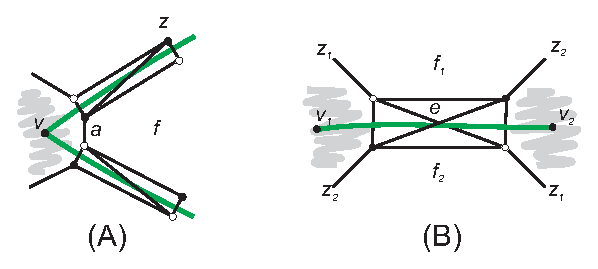
\includegraphics{A.figs/qialphabeta.eps}
   \end{center}
   \caption{ Elements for the quantum invariant}
   \label{fig:qialphabeta}
\end{figure}

An edge $e$ of the blink $B$ corresponds in $G_B$ to a schema like
the one on Figure~\ref{fig:qialphabeta}B. In this situation, the
elements involved are the g-vertices $v_1$ and $v_2,$ the g-faces
$f_1$ and $f_2$ and the g-zigzags $z_1$ and $z_2.$ It is always
possible, for every edge $e$, to draw a schema like this and
follow this standard: the angle-edges of $z_1$ that appear on the
schema fall between $v_1$ and $f_1$ in one side and between $v_2$
and $f_2$ on the other side. We now define
$$ \beta(e,x) = \left\{
\begin{array}{ll}
    {\displaystyle \frac{{\rm Tet}(x_{f_1},x_{v_1},x_{f_2},x_{v_2},x_{z_2},x_{z_1}) \,\,
                          \lambda(x_{f_1},x_{z_1},x_{v_1}) }
                        { \lambda(x_{v_2},x_{z_1},x_{f_2}) }}, & \hbox{\footnotesize if $e$ is green}
    \\[0.3cm]
    {\displaystyle \frac{{\rm Tet}(x_{f_1},x_{v_1},x_{f_2},x_{v_2},x_{z_2},x_{z_1}) \,\,
                          \lambda(x_{v_2},x_{z_1},x_{f_2}) }
                        { \lambda(x_{f_1},x_{z_1},x_{v_1}) }}, & \hbox{\footnotesize if $e$ is red}
    \\[0.1cm]
\end{array}\right.,$$
where ${\rm Tet}:{\cal I}^6 \rightarrow \mathbb{R}$ is defined as
$${\rm Tet}(a,b,c,d,e,f) = \frac{{\rm Int}!}{{\rm Ext}!} \sum_{m \leq s \leq
M}{\frac{(-1)^s[s+1]!}{\prod_{1 \leq i \leq 4}{[s-a_i]!\prod_{1\leq
j \leq 3}{[b_j-s]!}}}},
$$
in case the triples $(a,b,f)$, $(b,c,e)$, $(c,d,f)$, $(a,d,e)$ are
$r$-admissible and considering
$$\begin{array}{rcl}
{\rm Int}!&=&\prod_{1 \leq i \leq 4 \atop 1 \leq j \leq 3}[b_j-a_i]!\\ [0.2cm] {\rm Ext}!&=&[a]![b]![c]![d]![e]![f]!\\
[0.2cm] a_1&=&\frac{1}{2}(a+b+f)\qquad b_1=\frac{1}{2}(b+d+e+f)\\
[0.2cm] a_2&=&\frac{1}{2}(b+c+e)\qquad b_2=\frac{1}{2}(a+c+e+f)\\
[0.2cm] a_3&=&\frac{1}{2}(c+d+f)\qquad b_3=\frac{1}{2}(a+b+c+d)\\
[0.2cm]
a_4&=&\frac{1}{2}(a+d+e)\qquad m\!=\!\max\{a_i\}\quad M\!=\!\min\{b_j\}.\\
\end{array}.$$
In case any of the triples is not $r$-admissible, the value of ${\rm
Tet}$ is zero. The function $\lambda: {\cal I}^3 \rightarrow \mathbb{C}$ is
defined by
$$ \lambda(a,b,c) =
\left\{%
\begin{array}{ll}
    (-1)^{(a+b-c)/2}A^{[a(a+2)+b(b+2)-c(c+2)]/2}, & \hbox{\footnotesize if $a,b,c$ is $r$-admissible;} \\
    0, & \hbox{\footnotesize otherwise.} \\
\end{array}%
\right.$$ Finally, the function ${\rm wrt}_M$ is defined as
$$ {\rm wrt}_M(r) = \frac{{\rm raw}_M(r)}{{\rm raw}_{S_1 \times
S_2}(r)}$$

Note that ${\rm wrt}$ is normalized by the raw values of the space
$\mathcal{S}^2 \times\mathcal{S}^1$. The Figure~\ref{fig:qinvariante} presents the
values of the quantum invariant to the Poincar� Sphere, $E$, for $3 \leq r \leq 30$.

\begin{figure}[htp]
   \begin{center}
      \leavevmode
      %\includegraphics{A.figs/blinkgraphlbl.\jpgext}

\begin{footnotesize}
\begin{tabular}{|rrclr|} \hline
 $r$ & \multicolumn{3}{c}{${\rm wrt}_E(r)$} & ev \\[0.1cm] \hline
 3 & 0.7071067811 & + & 0.0000000000$i$ & 2 \\
 4 & -0.5000000000 & + & 0.0000000000$i$ & 4 \\
 5 & -0.3007504775 & - & 0.9256147934$i$ & 6 \\
 6 & 0.2886751346 & + & 0.0000000000$i$ & 9 \\
 7 & -0.8460344491 & - & 0.0447830425$i$ & 12 \\
 8 & 0.0000000000 & - & 0.7325378163$i$ & 16 \\
 9 & -0.1761268770 & + & 0.4020460816$i$ & 20 \\
 10 & -0.7663118960 & - & 0.5567581822$i$ & 25 \\
 11 & 0.2998611170 & - & 0.1557368892$i$ & 30 \\
 12 & -0.7886751345 & + & 0.1830127018$i$ & 36 \\
 13 & -0.1148609711 & - & 0.7426524382$i$ & 42 \\
 14 & -0.1074423864 & + & 0.3977522621$i$ & 49 \\
 15 & -0.7770955704 & - & 0.5344039501$i$ & 56 \\
 16 & 0.3141711649 & - & 0.1762214752$i$ & 64 \\ \hline
\end{tabular}
\begin{tabular}{|rrclr|} \hline
 $r$ & \multicolumn{3}{c}{${\rm wrt}_E(r)$} & ev \\[0.1cm] \hline
 17 & -0.7804263387 & + & 0.1428530500$i$ & 72 \\
 18 & -0.0590950525 & - & 0.7636697702$i$ & 81 \\
 19 & -0.1301847177 & + & 0.3730119013$i$ & 90 \\
 20 & -0.7085827791 & - & 0.6254313947$i$ & 100 \\
 21 & 0.3410488374 & - & 0.1495290291$i$ & 110 \\
 22 & -0.7854601781 & + & 0.0248114386$i$ & 121 \\
 23 & 0.0600389356 & - & 0.7749612722$i$ & 132 \\
 24 & -0.1814470028 & + & 0.3376768599$i$ & 144 \\
 25 & -0.5895059790 & - & 0.7441570346$i$ & 156 \\
 26 & 0.3666499557 & - & 0.0969412734$i$ & 169 \\
 27 & -0.7726037705 & - & 0.1263662241$i$ & 182 \\
 28 & 0.2079977942 & - & 0.7581679950$i$ & 196 \\
 29 & -0.2393556663 & + & 0.2887208942$i$ & 210 \\
 30 & -0.4276587373 & - & 0.8531721152$i$ & 225 \\ \hline
\end{tabular}
\end{footnotesize}
   \end{center}
   \vspace{-0.3cm}
   \caption{ Example of quantum invariant: Poincar�'s sphere}
   \label{fig:qinvariante}
\end{figure}
\begin{comment}


\end{comment}

By playing with computation of the quantum invariants from various
blinks we discovered a rather peculiar space.
\begin{conjecture}
The quantum invariants
of the space induced by the blink of Figure~\ref{fig:strange} are:
$q_r = \frac{2}{3}\,r$ if $r \equiv 0$ mod $3$, $q_r =
\frac{1}{3}\,(r+1)$ if $r \equiv 2$ mod $3$, $q_r =
\frac{1}{3}\,(r-1)$ if $r \equiv 1$ mod $3$.
\end{conjecture}
We have checked this
result to a precision of 10 decimal places and up to $r=45$. The
fact that the quantum invariants are real is evident since the blink
is red-green symmetric. The fact that they are all integer values
and that every integer appears is rather pleasing.
%-----------------------------------
    %\vspace{0.5cm}
    \begin{figure}[h!]
        \begin{center}
            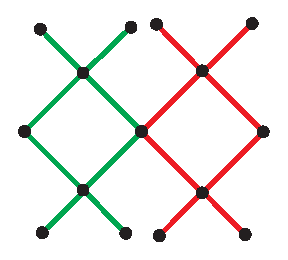
\includegraphics[width=4cm]{A.figs/strange.eps}
        \end{center}
        \caption{A peculiar space: its quantum invariants are integers and every integer appears}
        \label{fig:strange}
    \end{figure}
%-----------------------------------

\subsection{Code of a g-blink}
\label{sec:gblinkcode}

\newcommand{\pack}{\textsc{Pack}}
\newcommand{\reds}{\textsc{Reds}}
\newcommand{\GBlinkLabel}{\textsc{GBlinkLabel}}

In this section we are interested in defining a ``word'' with all
information of a g-blink, one that from it we are able to rebuild
the g-blink. This word is said to be the {\em code of the g-blink}.
Let $G$ be a g-blink. One of the ingredients to define this
``code'' is the \GBlinkLabel\ algorithm that labels the vertices of
a g-blink from an initial vertex $v$ (this initial vertex will be
labeled~1).
% \begin{algorithm}
% \begin{small}
% \caption{$\GBlinkLabel(G,v)$}
% \label{alg:maplabel}
% \begin{algorithmic}[1]
%  \State $S \leftarrow$ empty stack; $i \leftarrow 1$; $\forall u, L_u \leftarrow
%  \bot$ \Comment{$\bot$ = not defined}
%  \State push $v$ into $S$
%  \While{$S$ not empty}
%     \State $a \leftarrow$ pop $S$
%     \If{$L_a = \bot$}
%        \State $b \leftarrow {\rm adj}_f(a)$; $c \leftarrow {\rm adj}_v(b)$; $d \leftarrow {\rm adj}_v(a)$
%        \State $L_a \leftarrow i; L_b \leftarrow i+1; L_c \leftarrow i+2; L_d \leftarrow i+3$
%        \State push ${\rm adj}_a(b)$ into $S$; push ${\rm adj}_a(d)$ into $S$
%        \State $i \leftarrow i+4$
%     \EndIf
%  \EndWhile
%  \State {\bf return} $L$
% \end{algorithmic}
% \end{small}
% \end{algorithm}

When we talk about a {\em labeling of a g-blink or of a blink}, we
are referring to a labeling of the vertices of the g-blink given by
{\GBlinkLabel} with a starting vertex being some vertex with parity
1 in $G$. With this constraint, the set of vertices with even label
defined by {\GBlinkLabel}  is exactly the set $V_0$ of $G$ and the
set of vertices with odd label is exactly the set $V_1$ of $G$.
Other important properties of a labeling are: adjacent vertices by
face, vertex or angle edges in $G$ have labels with different
parity; the vertices of the same g-edge have labels $4k-3$, $4k-2$,
$4k-1$, $4k$ for some $k \geq 1$. From the label of a vertex it is
possible to know the label of its neighbor by face, vertex and
zigzag edge. For instance, if $u$ has label $4k-2$ (for some integer
$k\geq 1$) then its neighbor by face edge has label $4k-3$, by
vertex edge has label $4k-1$ and by zigzag edge has label $4k$. One
consequence of this fact is that it is possible to rebuild all
edges of $G$ annotating only the angle edge's neighbors, once the
face edge, vertex edge and zigzag edge are all known from the vertex
label.

Let $L$ be a labeling for $G$. Let $a_1,a_2 \ldots, a_{4n}$ be the
labels of the adjacent vertices by angle edges of the vertices
$1,2,\ldots,4n$ under the $L$ labeling. As we saw, this list is
sufficient to restore the vertices and the edges of $G$. Note also
that, by the property that adjacent vertices have labels with
different parity, this list is made of even labels followed by odd
labels and that if $a_i = j$, then $a_j = i$. From these two
observations it follows that from $\frac{a_1}{2}, \frac{a_3}{2},
\ldots, \frac{a_{4n-1}}{2}$ it is possible to restore $a_1,a_2
\ldots, a_{4n}$ and, consequently, the vertices and edges of $G$. We
denote the list (with labels divided by 2) as the
{\em packed representation of $L$}. Note that the packed
representation is a permutation of $1,\ldots,2n$. If $L$ is a
labeling, we denote by $\pack(L)$ the packed representation of $L$.
\begin{figure}[htp]
   \begin{center}
      \leavevmode
      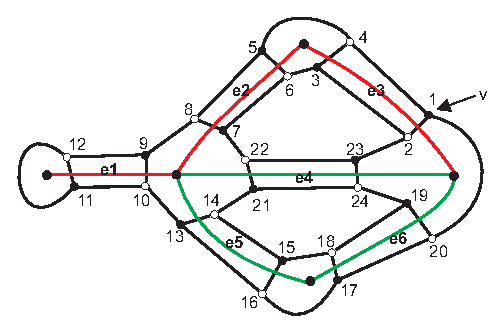
\includegraphics{A.figs/gblinklabeling.eps}
   \end{center}
   \vspace{-0.7cm}
   \caption{ blink $B$, g-blink $G_B$ and labeling $\textsc{GBlinkLabel}(G_B,v)$}
   \label{fig:gBlinkLabeling}
\end{figure}

The Figure \ref{fig:gBlinkLabeling} presents a blink $B$, its
induced g-blink $G_B$ and the labeling resulted of
${\GBlinkLabel}(G_B,v)$. In this case, the label of the adjacent
vertices by angle edge of $1,\ldots,24$ are $a_1,a_2,\ldots,a_{24}
=$ 20, 23, 6, 5, 4, 3, 22, 9, 8, 13, 12, 11, 10, 21, 18, 17, 16, 15,
24, 1, 14, 7, 2, 19. Its packed representation is $\frac{a_1}{2},
\frac{a_3}{2}, \ldots, \frac{a_{23}}{2} = $ 10, 3, 2, 11, 4, 6, 5,
9, 8, 12, 7, 1.

We represent the bicoloration of the g-edges of a g-blink under the
labeling $L$ by the set of integers $\reds(G,L)$ defined this way:
$k$ is in $\reds(G,L)$ if g-edge with vertices
$4k-3$, $4k-2$, $4k-1$ and $4k$ is red, otherwise $k$
is not in $\reds(G,L)$.

Let $L$ be a labeling for the g-blink $G$, then the {\em pre-code}
of $G$ for labeling $L$ is the pair $$(\pack(L),\reds(G,L)).$$
In the example of Figure \ref{fig:gBlinkLabeling}, the edges $e_1,$
$e_2,$ $e_3,$ $e_4,$ $e_5,$ $e_6$ are labeled with 3, 2, 1, 6, 4, 5
respectively. It follows that the {\em pre-code} for this blink
under the presented labeling (starting at $v$, Figure
\ref{fig:gBlinkLabeling}) is: $$((10, 3, 2, 11, 4, 6, 5, 9, 8, 12,
7, 1),\{1,2,3\}).$$

It is easy to see that different labelings define different
pre-codes and that the same blink may have different labelings
by changing the vertex~1 on the procedure {\GBlinkLabel}. This creates a
difficulty: two different pre-codes for the same g-blink. To resolve
this we define the order relation $\preceq$  on the set of pre-codes. Let
$(\pi_1,R_1)$ and $(\pi_2,R_2)$ be two pre-codes, then
$$
(\pi_1,R_1) \preceq (\pi_2,R_2) \hbox{ if }
\left\{
\begin{array}{l}
  |\pi_1| < |\pi_2| \,\,\, \hbox{ or }\\
  |\pi_1| = |\pi_2| \hbox{ and } \pi_1 < \pi_2 \,\,\, \hbox{ or }\\
  \pi_1 = \pi_2 \hbox{ and } |R_1| < |R_2| \,\,\, \hbox{ or }\\
  \pi_1 = \pi_2 \hbox{ and } R_1 = R_2 \,\,\, \hbox{ or }\\
  \pi_1 = \pi_2 \hbox{ and } |R_1| = |R_2| \hbox{ and } \min(R_1 \backslash R_2) < \min(R_2 \backslash R_1),\\
\end{array}
\right.
$$
where $|\pi|$ is the length of the permutation $\pi$ and $|R|$ is
the size of set $R$. The {\em code of the g-blink} $G$ is its greatest pre-code under
the relation $\preceq$:

\newcommand{\MaxPreCode}{\lower1.5ex\hbox{$\buildrel {\displaystyle max} \over {\scriptstyle \preceq}$}}

$$ \kappa(G) =
   \MaxPreCode \left\{
(\, \pack(L_v),\reds(G,L_v)\,)  \, \left|
\begin{array}{l}
      L_v = \GBlinkLabel(G,v), \\
      v \in V_1[G]
\end{array} \right. \right\}.$$
The {\em code of a blink $B$} is defined as
$\kappa(B) = \kappa(G),$ where $G$ is the induced g-blink of $B$.
A labeling $L$ of a g-blink is said to be a {\it code labeling of $G$}
if $(\,\pack(L),\reds(G,L)\,) = \kappa(G)$. We extend the relation
$\preceq$ on pre-codes to g-blinks and blinks in this natural way:
g-blink $G_1$ {\it is smaller or equal to} g-blink $G_2$, $G_1 \preceq G_2$,
if $\kappa(G_1) \preceq \kappa(G_2)$; blink $B_1$ {\it is smaller
or equal to} blink $B_2$, $B_1 \preceq B_2$, if their induced g-blinks
satisfy $G_1 \preceq G_2$.


\subsection{\textsc{Dual}, \textsc{Reflection} and \textsc{RefDual}
of a g-blink} \label{sec:dualReflectionRefDual}

In this section we study the effects of simple changes on the structure
of a g-blink. For instance, what happens to the induced space of a g-blink
if we swap the parity of its vertices? And what happens to its blink
presentations if we do this? We are interested in studying three types of
modifications in the structure of a g-blink. One of them is swapping the
parity of the vertices and we denote it by (P). Before naming the
other two we establish the convention we use to encode g-blinks.

We saw in the definition of g-blinks that we may encode the red-green
coloring of the \hbox{g-edges} directly or, alternatively, we may encode it by
registering the overcross/undercross status of the zigzag-edges of each
g-edge. In this section we assume that we are using this second
alternative. So, here, the color of the g-edges is a consequence of the
overcross/undercross state of the zigzag-edges of the g-blink.

Besides (P), the other two modifications in the structure of a g-blink that
we study are: swapping the role of face-edges with vertex-edges, denoted
by (FV); and swapping the overcrossing/undercrossing state of each
zigzag-edge, denoted by (C).

The central blink in Figure~\ref{fig:blinkWith8Operations} is a blink
presentation for our reference g-blink. By applying all combinations of
(P), (C) and (FV) on this g-blink we obtain new g-blinks
inducing the blinks shown. We can learn from this figure the effects
on blinks of these g-blink modifications. Applying (C), i. e. changing the
undercross/overcross status on the zigzag-edges, the only effect is
to swap the colors of the edges of the blinks; applying (P), i. e.
changing the parity of the vertices, the effect is to do
one reflection of the blink drawing and change the color of
its edges; applying (C) and (P), i. e. changing the undercross/overcross
state of each zigzag-edge and the parity of the vertices,  the effect
is just a reflection of the blink drawing; applying (FV), i. e. swapping
the roles of face-edge and vertex-edge, the blink becomes
the dual of the original blink (the dual is in the sense of a dual map or
dual plane graph) whose dual edges preserve
the same color as the original edges, followed by a
reflection; applying (C) and (FV), i. e. swapping the roles of face-edge and vertex-edge and
changing the overcross/undercross status of the zigzag-edges, the effect is
a dual blink with the dual edges having changed color (for instance, a dual edge that
``crosses'' a red edge becomes a green one) followed by a reflection;
applying (P) and (FV) the effect is the dual blink with dual edges
having the changed colors (for example, a dual edge that
``crosses'' a red edge becomes a green one); applying (C), (P) and (FV),
i. e. all three modifications, the effect is the dual of the blink with
the dual edges having the same color as the original ones (for example, a dual edge
that crosses a green edge is itself a green edge).
\begin{figure}[htp]
   \begin{center}
      \leavevmode
      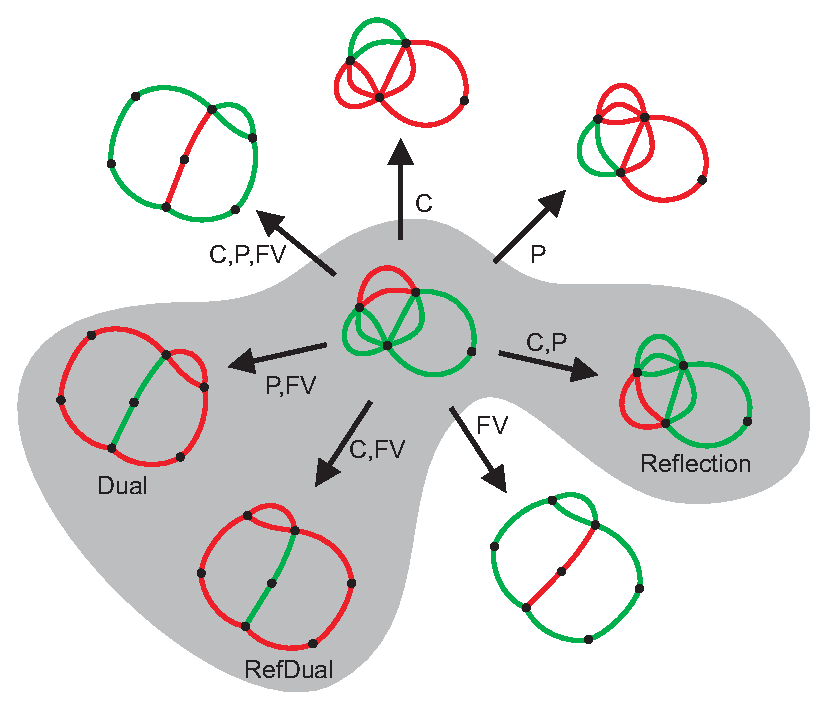
\includegraphics[width=10cm]{A.figs/blinkwith8operations.eps}
   \end{center}
   \vspace{-0.7cm}
   \caption{The effect on blinks of applying all combinations of (C), (P)
   and (FV) on its g-blink}
   \label{fig:blinkWith8Operations}
\end{figure}
Note that the blinks (and g-blinks) differing by the application of
two distinct modifications have special names. If $G$ is a g-blink,
the g-blink obtained from $G$ by applying (C) and (P) is said to be
the {\it reflection} of $G$ and is denoted by \textsc{Reflection}($G$);
the g-blink obtained from $G$ by applying (C) and (FV) is said to be
the {\it refdual} of $G$ and is denoted by \textsc{RefDual}($G$); the
g-blink obtained from $G$ by applying (P) and (FV) is said to be
the {\it dual} of $G$ and is denoted by \textsc{Dual}($G$). They
were shown in Figure~\ref{fig:blinkWith8Operations} over a gray
region because they all share one important property as the next
proposition shows.

\begin{proposition}\label{prop:dualGblink}
The spaces induced by g-blinks $G$, \textsc{Reflection($G$)},
\textsc{RefDual($G$)} and \textsc{Dual($G$)} are the same.
\end{proposition}

\vspace{-0.5cm}

\begin{proof}
$(G \equiv_S \textsc{Dual}(G))$ -- Consider the dual g-blinks on
Figure~\ref{fig:dualGBlinksInduceSameSpace}A and
Figure~\ref{fig:dualGBlinksInduceSameSpace}D. Following the drawings
in each row of this figure we see how to obtain one induced BFL from
a g-blink. Now observe that the BFLs on
Figure~\ref{fig:dualGBlinksInduceSameSpace}C and
Figure~\ref{fig:dualGBlinksInduceSameSpace}F induce the same space
because we can get from one to the other by applying, on $e$, the
space preserving move for BFLs of Lemma \ref{lem:jumpingRopeLemma}
(Jumping Rope Lemma for BFLs). It is easy to see that this argument
generalizes to any pair $G$ and  $\textsc{Dual}(G)$, so
$G \equiv_S \textsc{Dual}(G)$.
\begin{figure}[htp]
   \begin{center}
      \leavevmode
      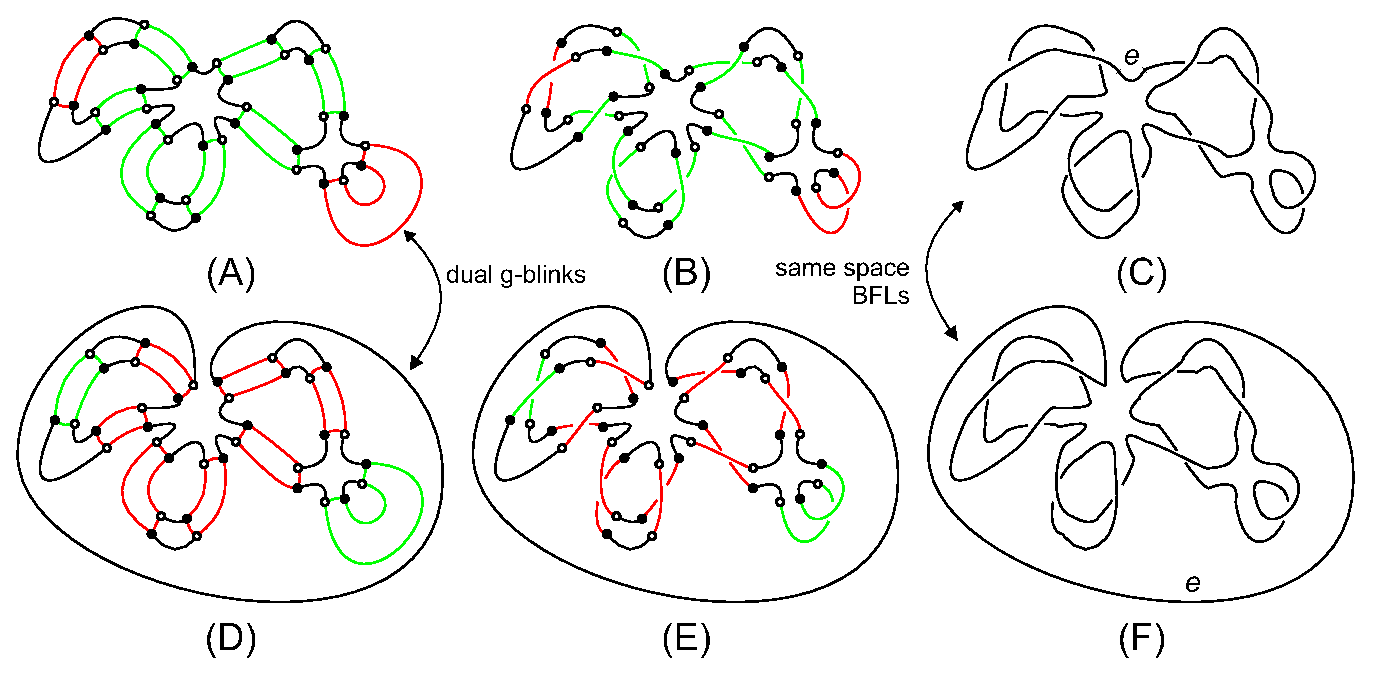
\includegraphics[width=13cm]{A.figs/dualgblinksinducesamespace.eps}
   \end{center}
   \vspace{-0.7cm}
   \caption{Dual g-blinks induce the same space}
   \label{fig:dualGBlinksInduceSameSpace}
\end{figure}


$(G \equiv_S \textsc{Reflection}(G))$ --
We prove the result in BFL language. Consider a plane disk $D^2$
containing the BFL. Do a $3D$-flip of $D^2$ carrying the BFL along.
Clearly this maintains the ambient isotopy link associated to the
BFL. The writhe of the components do not change: the blink has been
reflected but also its crossings are switched, thus maintaining all
crossing signs. The Proposition is established.

$(G \equiv_S \textsc{RefDual}(G))$ -- Note that
$\textsc{RefDual}(G) = \textsc{Reflection}(\textsc{Dual}(G))$, once applying
(P) and (FV) followed by (P) and (C) is the same as applying only (FV) and (C).
So, by the transitivity of the $\equiv_S$ relation, using the previous two results,
$G \equiv_S \textsc{RefDual}(G)$.
\end{proof}

What about the blinks that did not fall in the gray region of
Figure~\ref{fig:blinkWith8Operations}? What spaces do they induce?
First, it is easy to see that they all induce the same space once,
taking as reference the top most blink (north), the northeast
blink is its reflection (i. e. to get there we must apply (C) and (P)),
the southeast blink is its refdual and the northwest blink is its dual.
So, by Proposition~\ref{prop:dualGblink} they induce the same space.
To finish the answer, let's focus again on the top most blink (result
of (C) operation). It is obtained from the central blink by changing
crossing status of the zigzag-edges. In the blink view of the g-blink
this is equivalent to swap the colors of the edges from green to
red and vice-versa. On the BFL view this is just that: change all
the crossings. This has the effect of inverting the writhe of all
components: for example, a component that had writhe 1 becomes one
with writhe -1. So the end effect of this change
is to invert the orientation of the original space. Conclusion:
the g-blinks on the white region of Figure~\ref{fig:blinkWith8Operations}
induce the same space of the gray region g-blinks except for the
orientation that is changed.

\newcommand{\summaryOfInterpretations}{
{ \small \setstretch{1.1}
% parskip
\setlength{\parskip}{-2pt} \sl
\begin{tabular}{|ccc|} \hline
\multicolumn{3}{|c|}{\textsc{Dual($G$)}} \\
g-blink & blink & BFL \\ \hline
\multicolumn{1}{|p{4.5cm}|}{\protect \centering change parity (P) and swap face-edges and vertex-edges (FV) \\[0.3cm] 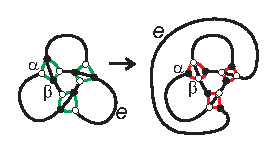
\includegraphics{A.figs/smallgblinkdual.eps}} &
\multicolumn{1}{|p{4.5cm}|}{\protect \centering each face becomes a
vertex, each
edge becomes a dual edge with different color \\[0.3cm] 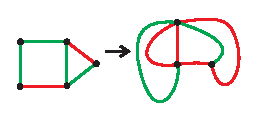
\includegraphics{A.figs/smallblinkdual.eps}} &
\multicolumn{1}{|p{4.5cm}|}{\protect \centering overpass one external edge \\[0.3cm] 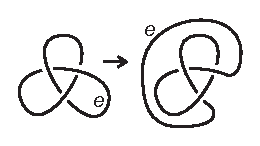
\includegraphics{A.figs/smallbfldual.eps}} \\ \hline
\multicolumn{3}{|c|}{\textsc{Reflection($G$)}} \\[0.1cm]
g-blink & blink & BFL \\ \hline \multicolumn{1}{|p{4.5cm}|}{\protect
\centering change parity (P) and change overcross and undercross
status on zigzag-edges (C) \\[0.3cm]
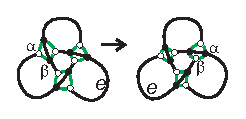
\includegraphics{A.figs/smallgblinkreflection.eps}}  &
\multicolumn{1}{|p{4.5cm}|}{\protect \centering
reflect \\[0.3cm] 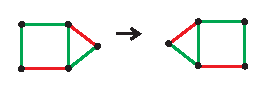
\includegraphics{A.figs/smallblinkreflection.eps}} &
\multicolumn{1}{|p{4.5cm}|}{\protect \centering
reflect and change the crossings  \\[0.3cm]
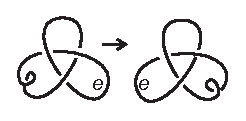
\includegraphics{A.figs/smallbflreflection.eps}} \\ \hline
\multicolumn{3}{|c|}{\textsc{RefDual($G$)}} \\
g-blink & blink & BFL \\ \hline \multicolumn{1}{|p{4.5cm}|}{\protect
\centering change overcross and undercross
status on zigzag-edges (C) and swap face-edges and vertex-edges (FV) \\[0.3cm]
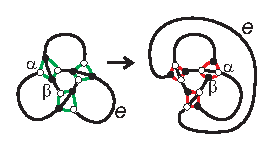
\includegraphics{A.figs/smallgblinkrefdual.eps}} &
\multicolumn{1}{|p{4.5cm}|}{\protect \centering first make each face
become a vertex and each
edge become a dual edge with the color changed, then reflect
the result \\[0.3cm]
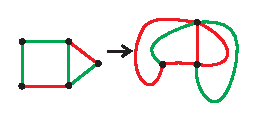
\includegraphics{A.figs/smallblinkrefdual.eps}} &
\multicolumn{1}{|p{4.5cm}|}{\protect \centering overpass one
external edge, reflect and change the crossings \\[0.2cm]
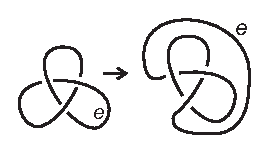
\includegraphics{A.figs/smallbflrefdual.eps}} \\[0.3cm] \hline
\end{tabular} \bigskip \medskip}}

One important consequence of the properties we described here is that we
may search for distinct spaces on only one of the eight possible g-blinks.
The other orientation of the space is trivially obtained from any g-blink.
This saves computational effort of identifying distinct spaces.

We end this section by summarizing the effects on the structures of
a g-blink, blink and BFL when the dual, reflection
and refdual operations are applied.

\subsection{Merging and breaking g-blinks} \label{sec:mergingGBlinks}

Let $A$ and $B$ be distinct g-blinks. A {\it basepair on $A$ and $B$}
is a pair of angle-edges $(a,b)$ so that $a \in A$ and $b \in B$. The
{\it merging of $A$ and $B$ at basepair $(a,b)$}, denoted by $$ A[a] + B[b] \,\,
,$$ is the g-blink obtained by replacing $a$ and $b$ by new edges
$e$ and $e'$ both connecting $A$ to $B$, having the
same ends as $a$ and $b$ and linking vertices of distinct parity.
See Figure~\ref{fig:merging} for an example.

\begin{figure}[htp]
   \begin{center}
      \leavevmode
      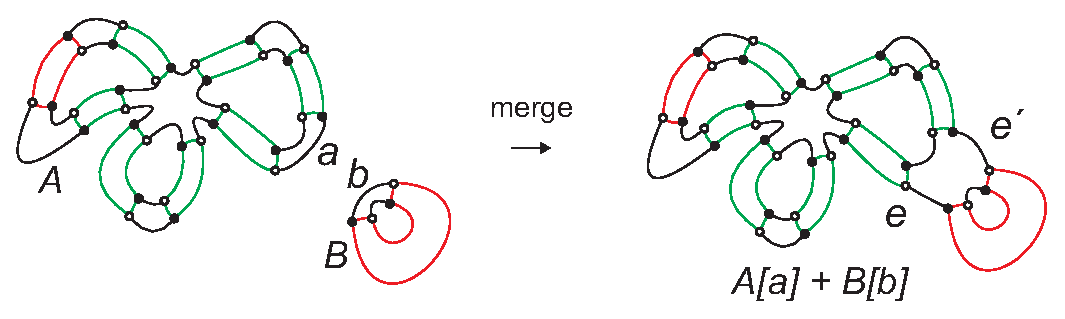
\includegraphics[width=14cm]{A.figs/merging.eps}
   \end{center}
   \vspace{-0.7cm}
   \caption{Merging of $A$ and $B$ on {\it basepair} $(a,b)$}
   \label{fig:merging}
\end{figure}

Observe the result of the merging of Figure~\ref{fig:merging}. The edges $e$
and $e'$ are both incident to the same g-face and g-vertex and we could reverse
the merging by replacing $e$ and $e'$ back with $a$ and $b$. Indeed, any pair of
distinct angle-edges incident to the same g-face and g-vertex on a g-blink
defines a {\it breakpoint}: a point where we can break a g-blink into two
disconnected g-blinks. To {\it break} a g-blink on {\it breakpair} $(e,e')$
is to separate it into two g-blinks by replacing edges $e$ and $e'$
by two new edges incident to same vertices of $e$ and $e'$ obtaining
two disconnected g-blinks. For an example see Figure~\ref{fig:merging}
from right to left.

\begin{theorem}[Theorem on partial dual]
\label{theo:partialDual} Let $A$ and $B$ be arbitrary disjoint
g-blinks and $(a,b)$ a basepair on them. Then
 $A[a] + B[b] \equiv_S A[a] + \textsc{Dual}(B)[b]$.
\end{theorem}
In the language of BFLs the diagrammatic reformulation of Theorem
\ref{theo:partialDual} is given by the diagram below. Note that
$\alpha$ and $\beta$ are the ends of $a$ and $\gamma$ and $\delta$
are the ends of $b$.
$$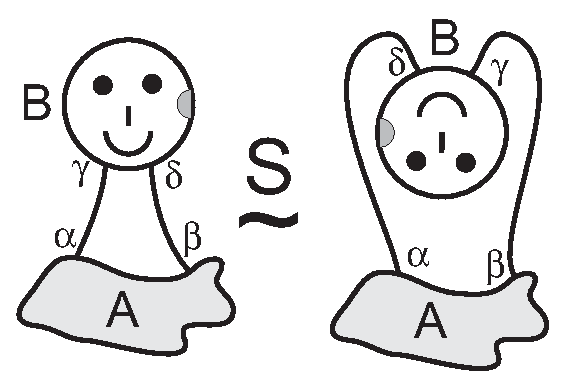
\includegraphics[width=5cm]{A.figs/partialdual.eps}$$ The right
diagram above is obtained by cutting the two wires $\pi$-rotating
$B$ and reconnecting the wires. (Note that the smiling fellow has
only the right rear.) Theorem~\ref{theo:partialDual} was suggested by
computer experiments very early in our research. It is a central
result to curtail the number of relevant blinks: see next section.
Its proof, however, was elusive until October 31, 2006: it has to
wait for the proofs of Theorems \ref{theo:partialReflection} and
\ref{theo:partialRefDual}.

\begin{theorem} [Theorem on partial reflection] \label{theo:partialReflection}
Let $A$ and $B$ be arbitrary disjoint g-blinks, $(a,b)$ a basepair
on them. Then $\, A[a] + B[b] \equiv_S A[a] +
\textsc{Reflection}(B)[b].$
\end{theorem}

In the language of blinks the diagrammatic reformulation of Theorem
\ref{theo:partialReflection} is on the left part of the diagram
below. The right part of it is the reformulation of the same Theorem
in BFL language. Note that the right ear becomes a left ear
indicating a $B$-reflection.
$$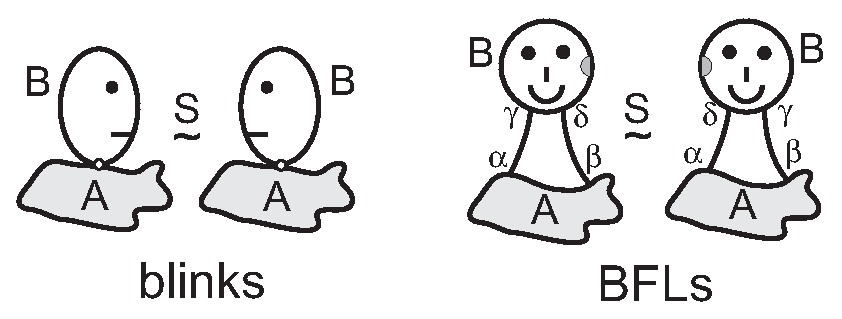
\includegraphics[width=10cm]{A.figs/partialreflection.eps}$$
Theorem \ref{theo:partialReflection} is proved by topological
techniques allied to crucial facts on the theory of gems. It is done
in Chapter 4. The proof of Theorem \ref{theo:partialReflection} is
the main theoretical contribution of this thesis.

The diagrammatic reformulation of Theorem
\ref{theo:partialRefDual} in the language of BFLs is the passage
from the first to the third diagram below
$$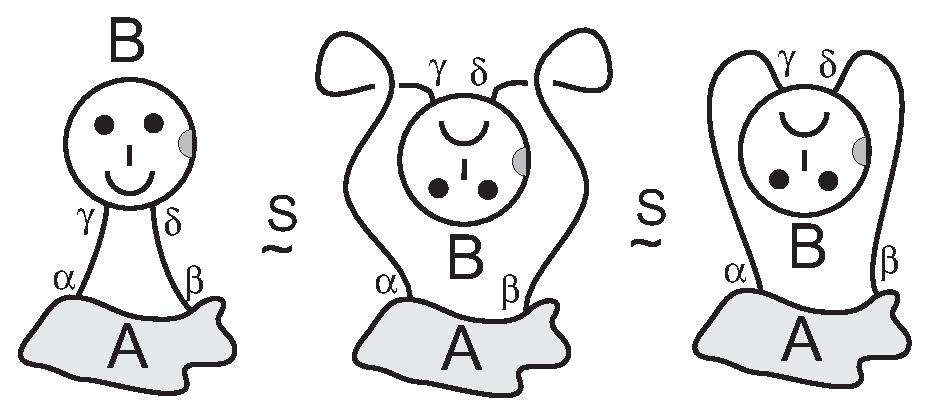
\includegraphics[width=8cm]{A.figs/partialrefdual.eps}$$ The third
diagram above is obtained by a $3D$-flip on $B$ (getting the central
diagram) followed by a ribbon move, regular isotopies and Whitney
trick. The smiling to frowning change is to indicate that all the
crossings are switched (and that the fellow became angry for being
put upside down and being retracted from the ear). On the contrary
of the previous Theorems we can tackle the proof of Theorem
\ref{theo:partialRefDual} immediately.

\begin{theorem}[Theorem on partial refDual]
\label{theo:partialRefDual} Let $A$ and
$B$ be arbitrary disjoint g-blinks, $(a,b)$ a basepair on them. Then
$A[a] + B[b] \equiv_S A[a] + \textsc{RefDual}(B)[b].$
\end{theorem}

\begin{proof}
The proof is easy with the help of the BFL manifestation of the
Theorem. See Figure \ref{fig:smilingFrowningFellow2}. The ambient
isotopy classes of the links corresponding to $A[a] + B[b]$ and to
$A[a] + \textsc{RefDual}(B)[b]$ are the same. It is enough to prove
that the writhe of each component of the BFLs is maintained. Outside
the $B$ there is no change in the crossing numbers. In the interior
of $B$ the crossings are switched and reflected (become upside down)
thus, again, there is no change in the crossing numbers. Finally,
the crossing numbers of the new curls are in the same component and
cancel each other.
\end{proof}

\begin{figure}[htp]
   \begin{center}
      \leavevmode
      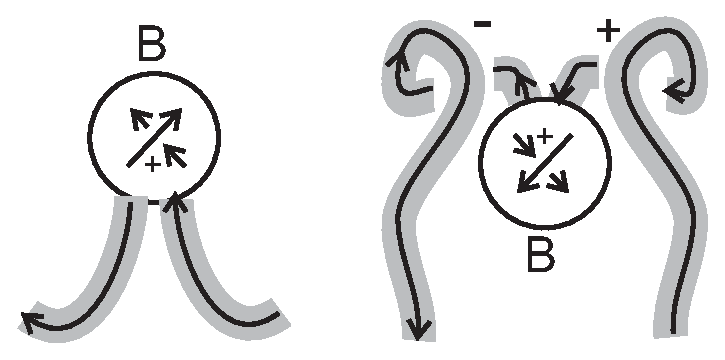
\includegraphics[width=8cm]{A.figs/smilingfrowningfellow2.eps}
   \end{center}
   \vspace{-0.7cm}
   \caption{BFLs induce same space because are the same link with the same
   writhe at each component}
   \label{fig:smilingFrowningFellow2}
\end{figure}

\begin{lemma} For any g-blink $B$,
$$\textsc{Dual(Reflection}(B))=\textsc{Reflection}(\textsc{Dual}(B)).$$
\end{lemma}
\begin{proof} By their combinatorial definitions in g-blinks
the operations of taking the dual and reflecting are seen to be
commuting involutions. Thus, both spaces in the statement of the
lemma are equal to $\textsc{RefDual}(B))$.
\end{proof}

\begin{lemma} \label{lem:23implies1}
Theorem \ref{theo:partialDual} is implied by Theorems
\ref{theo:partialReflection} and \ref{theo:partialRefDual}.
\end{lemma}
\begin{proof}
$A[a] + B[b] \equiv_S A[a] + \textsc{Reflection}(B)[b]$ and $A[a] +
B[b] \equiv_S A[a] + \textsc{RefDual}(B)[b]$ imply by transitivity
that $A[a] + \textsc{Reflection}(B)[b] \equiv_S A[a] +
\textsc{RefDual}(B)[b]$. Note that $b$ is an angle-edge in $C
=\textsc{Reflection}(B)$. Taking $c=b$ we have for any blink $C$,
$A[a] + C[c] \equiv_S A[a] + \textsc{Dual}(C)[c]$, establishing
Theorem \ref{theo:partialDual} for arbitrary disjoint g-blinks
$(A,C)$ and basepairs $(a,c)$.
\end{proof}
From Lemma \ref{lem:23implies1} and Theorem
\ref{theo:partialRefDual}, Theorem \ref{theo:partialDual} will
follow from Theorem \ref{theo:partialReflection}. The proof of this
result is given at the end of Chapter 4.

\subsection{Representative of a g-blink}
\label{sec:gblinkrepresentative}

We learned on Section \ref{sec:gblinks} that a g-blink induces
different blinks. All these blinks induce the same space, which is
defined as the space of the g-blink. We saw also that different
g-blinks may induce the same space: the g-blinks $G$,
$\textsc{Reflection}(G)$, $\textsc{Dual}(G)$ and $\textsc{RefDual}(G)$
dual are different g-blinks but induce the same space.
In this section we define a normalization procedure for g-blinks.
This normalization maps a g-blink into another g-blink that induces
the same space as the first. Our goal with this procedure is to look
for different spaces on fewer g-blinks: we need to look for different spaces
only on g-blinks that are normalized. The normalized version of a
g-blink will be denoted as its {\it representative}.

We saw on Section~\ref{sec:mergingGBlinks} that a breakpair on
a g-blink is a pair of angle-edges that are on
the same g-vertex and the same g-face. Given a g-blink and one
breakpair in it we may separate it into two g-blinks.
Figure~\ref{fig:breakpair}A shows a g-blink and its breakpairs: the
gray arrows point to the pair of angle-edges of the breakpair. We
can separate a g-blink in pieces (smaller g-blinks) until there are
no more breakpairs.
Figures~\ref{fig:breakpair}B, \ref{fig:breakpair}C and \ref{fig:breakpair}D
show this separation process. A piece without breakpairs is called a
{\it block}. Figure~\ref{fig:breakpair}D have 4 blocks. No matter
what sequence of breakpairs one uses to separate a g-blink in blocks,
the final blocks are always the same.
\begin{figure}[htp]
   \begin{center}
      \leavevmode
      
\includegraphics[width=14cm]{A.figs/breakpoint.eps}
   \end{center}
   \vspace{-0.7cm}
   \caption{Breakpoints of a g-blink and its breaking}
   \label{fig:breakpair}
\end{figure}

Some important properties of a breakpair that we need are related to
the g-zigzags of its g-blink. They are the subject of next two
propositions.

\begin{proposition}
If $p$ is a breakpair on g-blink $G$ and its angle-edges are $e_1$
and $e_2$ then the g-zigzag of $G$ that contains $e_1$ is the same
as the one that contains $e_2$.
\end{proposition}
\begin{proof} Straightforward. \end{proof}


\begin{proposition}
\label{prop:breakpairDisjointGZigzags}
 The only g-zigzag $z$ affected by separating a g-blink $G$ on
a breakpair $p$ is the one that contains both angle-edges of
$p$. If $P_1$ and $P_2$ are the pieces obtained by separating $G$ on
$p$ then the g-zigzags of $P_1$ and $P_2$, except for $z$, were
disjoint in $G$.
\end{proposition}
\begin{proof} Straightforward. \end{proof}

We also saw on Section~\ref{sec:mergingGBlinks} that any pair of angle
edges, each on different g-blinks may be the {\it
basepair} of a g-blink merging operation. Think of the
transition from Figure~\ref{fig:breakpair}B to
Figure~\ref{fig:breakpair}A the basepairs are the angle-edges labeled
1 on Figure~\ref{fig:breakpair}B. So, to merge two g-blinks on a
basepair is to replace the basepair angle-edges by two new edges
connecting the two g-blinks and respecting the parity.

\begin{figure}[htp]
   \begin{center}
      \leavevmode
      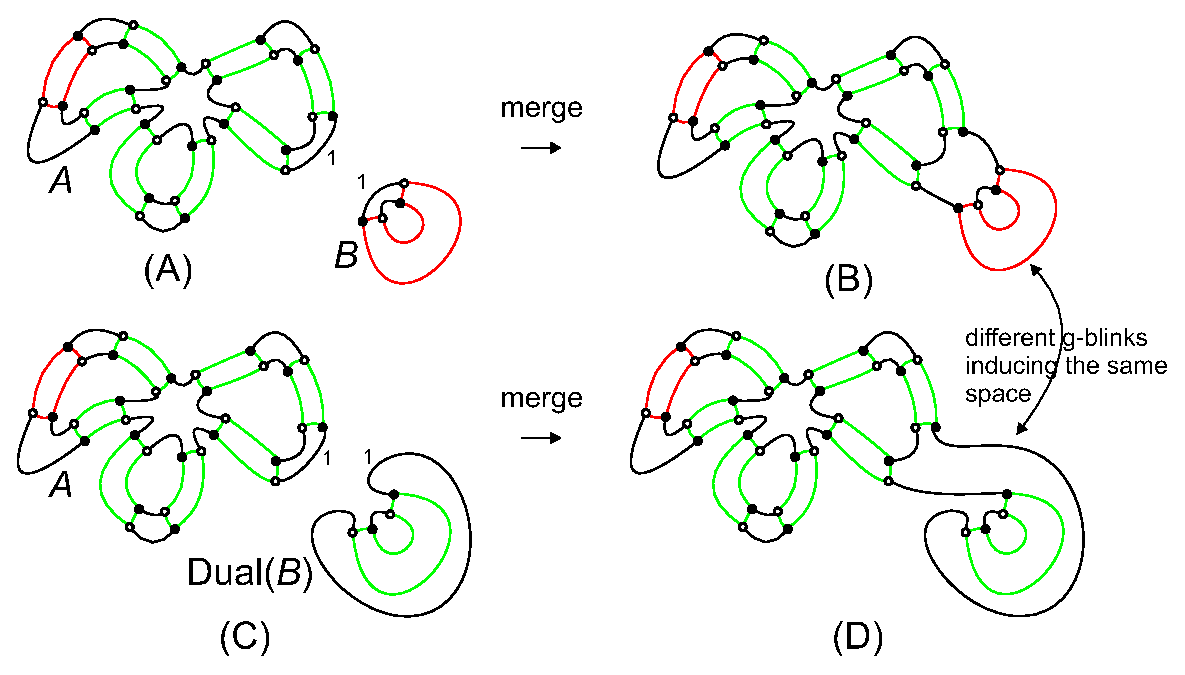
\includegraphics[width=14cm]{A.figs/mergingwithdual.eps}
   \end{center}
   \vspace{-0.7cm}
   \caption{Merging A with B and with \textsc{Dual}(B)}
   \label{fig:mergingWithDual}
\end{figure}

The fact that the two g-blinks at the right of Figure
\ref{fig:mergingWithDual} induce the same space is given by Theorem
\ref{theo:partialDual}. The proof of this Theorem still depends on
the proof of Theorem \ref{theo:partialReflection} which will be
given in Chapter 4. It depends on topological facts and a
reformulation of the BFL in terms of gems. As we have said before,
this is the main theoretical contribution of our Thesis.

Follow Figure~\ref{fig:mergingWithDual} to see an application of
Theorem \ref{theo:partialDual}. The basepair in both rows are the
same: the pair of edges labeled~1. The theorem together with the result
we describe now form the basis of the normalization procedure.

\begin{proposition} \label{prop:sameZigzagsSameSpace}
Let $A$ and $B$ be two g-blinks. Let $p$ be a basepair on them. Let $\alpha$
be the g-zigzag of the angle-edge of $p$ on $A$ and $\beta$ be the
g-zigzag of the angle-edge of $p$ on $B$. Let $p'$ be any other
basepair on g-zigzags $\alpha$ of $A$ and $\beta$ of $B$. The result
of $A$ and $B$ merged on $p$ induces the same space as $A$ and $B$
merged on $p'$.
\end{proposition}

For example, the g-blink resultant of the merge of
Figure~\ref{fig:mergingOnAnyAngleEdge}A on basepair labeled 1
induces the same space as the g-blink resultant of merging any pair
of angle edges tagged with a ``blue X'' one from $A$ and another
from $B$ of Figure~\ref{fig:mergingOnAnyAngleEdge}B. Note that all
angle-edges tagged with a ``blue X'' on
Figure~\ref{fig:mergingOnAnyAngleEdge}B are on the same g-zigzag of
the angle-edges labeled 1 on
Figure~\ref{fig:mergingOnAnyAngleEdge}A.
\begin{figure}[htp]
   \begin{center}
      \leavevmode
      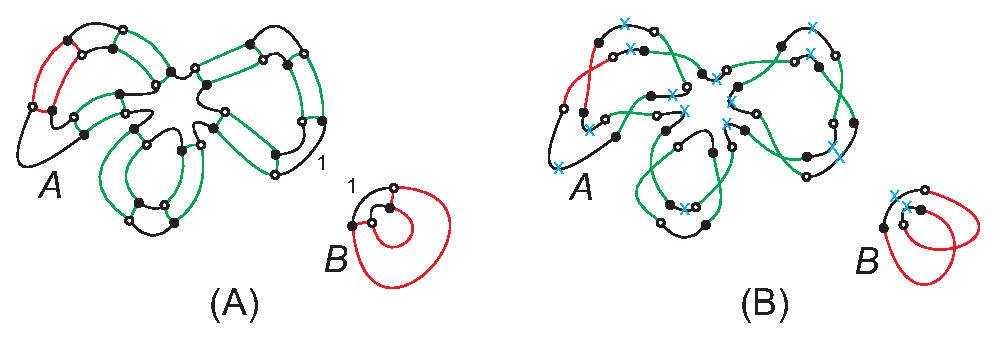
\includegraphics[width=12cm]{A.figs/mergingonanyangleedge.eps}
   \end{center}
   \vspace{-0.7cm}
   \caption{Merging on any angle-edge of the same g-zigzags}
   \label{fig:mergingOnAnyAngleEdge}
\end{figure}

Having Theorems \ref{theo:partialDual}, Theorem
\ref{theo:partialReflection} and Theorem \ref{theo:partialRefDual}
at our disposal, we are now able to describe the normalization
procedure. The intuitive idea is to separate the g-blink into blocks
and then remount the blocks (or their duals, reflection or refdual,
depending who is ``smaller'') in a canonical way. We divide this
procedure in three phases: separating phase, intermediate phase
and merging phase.

Separating phase. Let $G$ be the g-blink we want to normalize. First
give each g-zigzag of $G$ an unique label. Let $Z$ be the set of
these labels. For each angle-edge $e$ on $G$ record the label of the
g-zigzag that contains $e$ as its {\it zigzag label} $z_e$.
Initialize the ``pieces set'' as ${\cal P} \leftarrow \{G\}$.
Suppose there is a piece $P$ in ${\cal P}$ with a breakpair $p$. Let
$e_1$ and $e_2$ be the two angle edges of the breakpair $p$. Note
that the zigzag labels of $e_1$ and $e_2$ are the same: $z_{e_1} =
z_{e_2}$. Separate $P$ into $P_1$ and $P_2$ and make the two new
edges $e'_1$ on $P_1$ and $e'_2$ on $P_2$ have the same zigzag
labels as $e_1$ and $e_2$: $z_{e'_1} \leftarrow z_{e_1} (= z_{e_2})$
and $z_{e'_2} \leftarrow z_{e_1} (= z_{e_2})$. Replace $P$ with
$P_1$ and $P_2$ on ${\cal P}$. Repeat this until ${\cal P}$ contains
only blocks (g-blinks without breakpairs). The separating phase is
finished.

Intermediate phase. Define a bipartite graph $X$. The vertices of
$X$ are the labels $z \in Z$ and the pieces $P \in {\cal P}$; there
is an edge $(z,P)$ between label $z$ and piece $P$ in $X$ if there
is an angle-edge $e$ in $P$ with $z_e = z$. Note that $X$ is a tree:
no cycles. Let pieces $P_1$ and $P_2$ be neighbors of label $z$ on
$X$. The only common neighbor of $P_1$ and $P_2$ must be $z$
otherwise $P_1$ could not be separated from $P_2$ (See Proposition
\ref{prop:breakpairDisjointGZigzags}). This implies that there
cannot be a cycle in $X$. Remove every vertex $z \in Z$ of $X$ that
has only one neighbor. This asserts that every leaf of $X$ is a
vertex $P$ in ${\cal P}$. A consequence of this is that $X$ has a
single {\it center}. The center of a tree (see
\cite{BondyAndMurty1976}) is obtained by removing all leafs of a
tree in each step until arriving at a pair of vertices or a single
vertex. By applying the tree center algorithm on $X$ the leafs on
each step alternates between $z$ nodes and $P$ nodes. So it must
finish on a single node once there cannot be two adjacent $z$'s or
two adjacent $P$'s. Let $v$ be the center of $X$. We root $X$ at $v$
and $X$ becomes a {\it rooted tree}. The idea now is to organize
this rooted tree in a canonical way. To this aim we must have a way
to compare nodes and subtrees.

Remember from Section \ref{sec:gblinkcode} that every g-blink has a
unique code. So we can compare g-blinks by comparing their codes. We
know that merging a g-blink, or its dual, or its reflection or its refDual
on the same basepair results in a g-blink that induces the same space.
So we normalize ${\cal P}$ by replacing each piece $P$ in it by
$\min\{$ $P$, $\textsc{Dual}(P)$, $\textsc{Reflection}(P)$, $\textsc{RefDual}(P)$ $\}$.
Note that doing this does not affect the zigzag labeling of the angle-edges
because angle-edges are preserved on these operations (i. e. dual,
reflection and refdual). Note also that the
$P$ nodes of $X$ are also updated by this criterion. Using the code
of a g-blink we can also organize the rooted tree $X$. To organize
$X$ we mean to define a fixed sequence for the children of a node of
$X$. We do this inductively. The base case is a node without child.
This node is already organized, so we are finished. Consider a node
$u$ with children $w_1,\ldots,w_k$ all of them already organized. To
organize $u$ we need to define a sequence for these children. Using
the code of a g-blink we can define a function
\textsc{CompareTrees}($r_1$,$r_2$) to compare organized rooted trees
that is evaluated to -1 if tree rooted at $r_1$ is smaller than the
tree rooted at $r_2$, to 0 if they are the same and to +1 if tree
rooted at $r_1$ is greater than tree rooted at $r_2$. So to organize
$u$ is a matter of sorting $w_1,\ldots,w_k$ using the
\textsc{CompareTrees} function. With these explanations the problem
of organizing $X$ is solved. This also ends the intermediate phase.

% define the command: \CompareTreesAlgorithm
% \newcommand{\CompareTreesAlgorithm}{
% \parbox[t]{8cm}{
% \begin{small}
% \begin{algorithmic}[1]
%  \Statex
%  \Function {\textsc{CompareTrees}}{$r_1,r_2$}
%     \State $s_1 \leftarrow$ \textsc{LinearizeTree}($r_1$)
%     \State $s_2 \leftarrow$ \textsc{LinearizeTree}($r_2$)
%     \State $n_1 \leftarrow$ length($s_1$); $n_2 \leftarrow$ length($s_2$)
%     \State $i \leftarrow 1$
%     \While {$i \leq {\rm min}(n_1,n_2)$}
%        \State $(u_1,{\rm level}_1) \leftarrow s_1[i\,]$
%        \State $(u_2,{\rm level}_2) \leftarrow s_2[i\,]$
%        \State {\bf if} {$({\rm level}_1 < {\rm level}_2)$} {\bf then return} -1
%        \State {\bf else if} {$({\rm level}_1 > {\rm level}_2)$} {\bf then return} +1
%        \State {\bf if} {$\kappa(u_1) < \kappa(u_2)$} {\bf then return} -1
%        \State {\bf else if} {$\kappa(u_1) > \kappa(u_2)$} {\bf then return} +1
%        \State $i \leftarrow i + 1$
%     \EndWhile
%     \State {\bf if} {$n_1 = n_2$} {\bf then return} 0
%     \State {\bf else if} {$n_1 < n_2$} {\bf then return} -1
%     \State {\bf else} {\bf return} +1
%  \EndFunction
% \end{algorithmic}
% \end{small}}}
% % define the command: \LinearizeTreeAlgorithm
% \newcommand{\LinearizeTreeAlgorithm}{
% \parbox[t]{7.5cm} {
% \begin{small}
% \begin{algorithmic}[1]
%  \Statex
%  \Function {\textsc{LinearizeTree}}{$r$}
%     \State $s \leftarrow <>$
%     \Procedure {\textsc{LT-DFS}}{$u$,{\rm level}}
%        \State $s \leftarrow s \cdot <(u,{\rm level})>$
%        \For {every children $v$ of $u$ taken in the ordered sequence}
%            \State \textsc{LT-DFS}($v$,level+1)
%        \EndFor
%     \EndProcedure
%     \State \textsc{LT-DFS}($r$,0)
%     \State {\bf return} $s$
%  \EndFunction
% \end{algorithmic}
% \end{small}}}
% 
% \begin{algorithm}
% \caption{\textsc{CompareTrees} Algorithm}
% \label{alg:compareTrees}
% \begin{center}
% \CompareTreesAlgorithm \hspace{0.1cm} \LinearizeTreeAlgorithm

% \bigskip
% 
% \parbox{12cm}{
% \begin{small}
% In this algorithm the code $\kappa$ is taken over not only g-blinks
% but also on zigzag labels. Consider the code of a zigzag label the
% empty word. With this definition two zigzag labels $z_1$ and $z_2$
% always satisfy $\kappa(z_1) = \kappa(z_2)$. Note also that a zigzag
% node code is smaller than any g-blink code.\end{small}}
% \end{center}
% \end{algorithm}

Merging phase: The rooted tree $X$ is already organized. The idea
now is to merge the blocks using the order defined on $X$ and using
the code to define a canonical basepair for each merging operation.
Let $z$ be a label in $X$. Let $P_1, \ldots, P_k$ be the neighbors
of $z$. If $z$ is not the root of $X$ then $P_1$ is the parent of
$z$ and $P_2 \ldots P_k$ are the children of $z$ taken in order. If
$z$ is the root of $X$ then $P_1 \ldots P_k$ are the children of $z$
taken in order. We want now to merge the pieces $P_1 \ldots P_k$ in
the order they appear. First $P_1$ with $P_2$, second the result of
$P_1$ and $P_2$ with $P_3$ and so on. The only thing not defined yet
is the base point of each merging. This is solved using the code of
the blocks. For each label $z$ that appears on a block $P$ we define
a {\it canonical basepair angle-edge} $e_P^z$ on the g-zigzag whose
angle-edges are all zigzag labeled with $z$. This is done using the
code labeling of $P$ (see Section \ref{sec:gblinkcode}). Label the
vertices of $P$ with its code labeling. Define $e_P^z$ as the
angle-edge (among all angle-edges with zigzag label $z$ on $P$)
incident to the vertex of $P$ that has the smallest label.
The last thing we need to define is how to update the canonical
basepair angle-edge after a merging operation. In symbols, after
merging $P_1$ and $P_2$ whose canonical basepair angle-edges
were $e_{P_1}^z$ and $e_{P_2}^z$ what will be the canonical basepair
angle-edge $e_{P_1+P_2}^z$ of $P_1 + P_2$? By definition
$e_{P_1+P_2}^z$ will be the new angle-edge incident to the odd
vertex~of~$P_2$. Repeat this merging for all zigzag label $z$
in any order until no more merging may be
done. Finished.

This three-phase procedure results in a unique g-blink $r(G)$, {\it
the representative of $G$}. Both g-blinks, $G$ and $r(G)$ induce the
same space. A g-blink is said to be {\it a representative} if $G =
r(G)$. We finish this section with an example in
Figure~\ref{fig:dog} of the result of the algorithm that we have
implemented for obtaining the representative of a g-blink (or blink).
\begin{figure}[htp]
   \begin{center}
      \leavevmode
      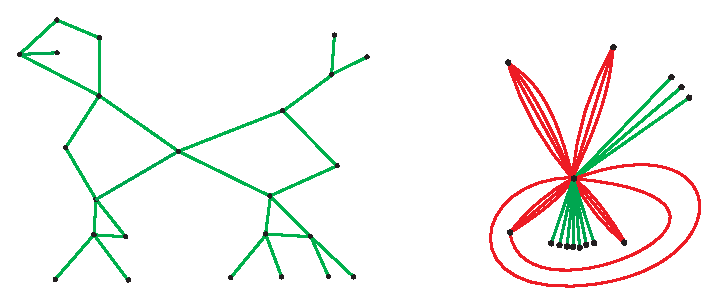
\includegraphics[width=12cm]{A.figs/dog.eps}
   \end{center}
   \vspace{-0.7cm}
   \caption{Representative of the dog like blink}
   \label{fig:dog}
\end{figure}

\subsection{Towards a census of spaces induced by small blinks}
\label{sec:towardsACensusOfPrimeSpacesInducedBySmallBlinks}

\begin{center}
\it What spaces have a small \underline{blink} presentation?
\end{center}
In this chapter we saw that a g-blink is a family of blinks that
induce the same space and that any blink has an associated g-blink.
Thus, our question is equivalent to
\begin{center}
\it What spaces have a small \underline{g-blink} presentation?
\end{center}
In this form, our original question becomes easier ``to be computed''
once a g-blink is a combinatorial object and the number of g-blinks
with $\,\,\leq k \,\,$ g-edges is finite. Moreover, by being
combinatorial simple objects, \hbox{g-blinks} have a direct way of
going into computers. For instance, a g-blink may be represented
in a computer by its code.

By the fact that every g-blink is associated to a special g-blink
with the same size that induces the same space called its
representative, our question is also equivalent to
\begin{center}
\it What spaces have a small \underline{representative g-blink}
presentation?
\end{center}
In this form, our original question becomes even ``easier'' in the sense
that, with $\,\,\leq k \,\,$ g-edges, there are fewer ``representative
g-blinks'' than ``general g-blinks''. Thus, this form is the one we
use.

Suppose we have generated the set of all representative g-blinks with
$\,\,\leq k \,\,$ g-edges for some $k \geq 1$. We already know that
all spaces that have a presentation with $\,\,\leq k \,\,$ edges are
there. But how to identify them? What elements of this set
(representative g-blinks) induce the same space? In
Sections~\ref{sec:homologyGroup}~and~\ref{sec:quantumInvariant} we
described a way to calculate two space invariants from a g-blink
presentation: the homology group and the quantum invariant.
Calculating these invariants on all g-blinks we can partition this
set in classes where each element of the same class has the same
homology group and same quantum invariant. At this point we are sure
that different classes induce different spaces because there is a
topological invariant that distinguishes them. The remaining problem
is to know if all g-blinks in the same class (same homology group
and same quantum invariant) induce the same space. To prove that two
\hbox{g-blinks} indeed induce the same space we will use a
computational method in 3-Gem Theory that was described in
\cite{lins1995gca}. Next chapter will be about 3-Gems and this
computational method.
